\documentclass{article}
\usepackage[utf8]{inputenc}
\usepackage{graphicx}
\usepackage[toc,page]{appendix}
\usepackage[nottoc]{tocbibind}
\usepackage[numbers]{natbib}
\usepackage{listings}
\usepackage{longtable}
\begin{document}
\graphicspath{ {images/} }

 \begin{center}
        
        \Huge
        \textbf{Distributed Chat System}
        
        \vspace{0.5cm}
        
        \Large
        By Hermes Team
        
        \vspace{1.5cm}

        \textbf{Khalil Jabir, Arsalan Ardeshiri, Yatharth Ranjan, Vashu Tyagi}
        
         \vspace{1.5cm}
         
        A report is presented for the module 7CCSMGPR Group Project\\
        as part of a Master of Science Degree
        
         \vspace{1.5cm}
        
        \Large
        Informatics\\
        King's College London\\
        England, UK\\
        30 March 2017\\
        
 \end{center}

\newpage
\begin{center}
\tableofcontents

\end{center}

\newpage
\section{Introduction}
\subsection{Context}
This project aims to deliver a distributed chat system which attempts to improve communications between users. The project researches and investigates a wide range of similar existing systems and focuses on the key features that such systems include so the proposed system will have all the core requirements that any chat system must at least have. In addition, the project aims to deliver a system which will be more efficient, reliable, user-friendly and secure.  \par
\subsection{Aims}

   \subsubsection {Primary Aims}
   \begin{itemize}
     \item \textbf{Provide and improve communications}: the main aim of this project is to deliver a distributed chat system which will enable users to communicate with each other in an efficient manner to improve communications. 
     \item \textbf{Enhance the level of use}: the second primary aim is to develop the system on two different platforms i.e. web and android applications. Not only that this will increase the number of users as some users may only use web applications while others may only use androids but also provide users with more flexibility in case they may wish to use the system on their PCs, laptops, tablets or mobile phones. 
   \end{itemize}
   
   \subsubsection {Secondary Aims}
   \begin{itemize}
     \item \textbf {Enhance throughput and process}: Once the primary aims are achieved, this secondary aim should be accomplished. This aim is all about allowing high throughput and enhancing the system so it still handles communications or exchange of messages efficiently with the lowest delay rate and in a time reasonable to the user which will help eliminate users’ inconveniences. This can also be accomplished by making the system user friendly compared to other systems e.g. adding communication symbols that can be used as alternatives of words which can make the system easier to use (improves usability). 
     \item \textbf {Implement and provide higher security}: this secondary aim focuses on the implementation of security features if it is to be achieved. Security features will include hashing of passwords and encryption and decryption of messages between end-to-end users. This will eliminate unauthenticated access and protect users’ messages and information from being accessed or potentially compromised. 
   \end{itemize}
   

\subsection{Objectives}
To achieve the above aims, certain objectives which are more specific must be accomplished as below: \par
\begin{itemize}
    \item Research and investigate a variety of distributed chat systems to better comprehend their functionality, characteristics, and architecture. 
    \item Use SWOT analysis technique to identify the group’s strength, weaknesses, opportunities, and threats which may have an impact on the project. 
    \item Identify and analyse potential risks that may arise during the project’s life cycle and set mitigation and contingency plan for each risk identified to help manage or overcome the risk. 
    \item Identify the system’s primary actors who are the actual users of the system and any secondary actors e.g. services that the system will interact with such as the database.
    \item Capture user stories (scenarios) to better understand the tasks that the target user may need to perform using the system. 
    \item Define the software system’s specifications, these are the functional requirements of the system which can be derived from the user stories captured. 
    \item Define the non-functional requirements which are the constraints under which the system will operate such as timing and security constraints. 
    \item Design a relational database schema which will be suitable to handle the data for the chosen platforms i.e. the website and android applications. 
    \item Design the wire-frame prototypes for both platforms to make the execution of the implementation phase smoother. 
    \item Plan the architecture of the system. This should include choice of technologies, platforms, resources, and design patterns. 
    \item Implement the relational database following the schema previously designed using MySQL. In addition, implement stored procedures to be used to avoid redundant queries that may be needed for both platforms.
    \item Implement the website pages using HTML5, CSS3 and use Java-Script where necessary. 
    \item Launch Android Studio and design the required screens for the Android app using Java and XML. 
    \item Implement the back-end functionalities for both platforms using PHP. The android app should also interact with the same server side as the website. Stored procedures implemented should be used by both platforms. 
    \item Perform appropriate unit or functional and usability testing as required. 
    \item Evaluate the entire process by identifying challenges, issues, failures or any weaknesses, justify the reasons behind them and list any intended future work. 
\end{itemize}

\subsection{Achievements}
We have implemented and delivered a distributed chat system with one server side and two clients i.e. Android and Web applications. The system was developed using a variety of different technologies such as HTML,CSS, PHP, Java-Script, XML and Java. The primary aims of this project have been achieved and core requirements that the system must have such as register, log-in, search user, initiate chat, send and receive message have been implemented as stated in the project's plan and tested to ensure correct functionality of the software system. In addition, some of the optional requirements such as search and delete chat were also implemented to enhance the system in terms of functionality and usability. \par

In addition, the secondary aims were partially achieved. For instance, the system is efficient as it enables users to send or receive a message within a few seconds time frame even though there is still more to improve in terms of efficiency and also users' passwords are all hashed before they are stored in the database meaning the system hashes passwords and authenticates users so no unauthenticated access is allowed. This means the system is secure even though we have not implemented the encryption/decryption of messages. 

\newpage
\section{Literature Review}
\subsection{Characteristics of a Distributed System}
As the project involves developing a distributed chat system which is a distributed software system, some characteristics of a distributed system were learnt to ensure the system is correctly developed. \par
There are some design features to consider when developing a distributed system as follows \cite{DS-Concepts}: \par
\begin{itemize}
    \item \underline{Openness}: the system should be implemented on published specifications e.g. standards to allow users interact with and use other systems from within the system if they wish to do so. 
    \item \underline{Concurrency}: the system will be multi-process which means multiple clients may try to access a service. Therefore, issues which are familiar with multi-process must be resolved e.g. locking and synchronisation. 
    \item \underline{Scalability}: the system is built as a small system at first using relatively cheap components but more components are added on demand as the system scales. Duplicated resources are necessary for the system’s scalability. 
    \item \underline{Fault tolerance}: the system should be able to tolerate faults using redundant hardware, and software recovery so even in the case of faults, the system will still be able to deliver the service. 
    \item \underline{Transparency}: the system should be transparent which means the user does not have to know specific information to use the system. 
    \item \underline{Security}: the system should be made secure by preventing users doing things they should not do and preventing actions which may accidentally prevent the correct functioning of the system. Security issues include authentication, confidentiality (e.g. data and traffic), and access control. 
    \item \underline{Performance}: the system should be responsive or able to process requests as quickly as possible, and able to allow as much as processing as possible referred to as a high throughput. 
    \item Other features include \underline{reliability} meaning the system should always be in a working order, be \underline{adaptable} to account for changes in use and technology over the time and \underline{time-critical} meaning it should meet strict timing constraints that certain operations may have. 
\end{itemize}

\subsection{Distributed Chat System Architecture}
\subsubsection{Facebook Messaging System Architecture}
The architecture of the system plays an important role for the system to be reliable and efficient. Therefore, the database must be designed in the most reliable and accurate way possible to prevent potential errors in the first place. However, as we are using agile methodology for managing the project, we will design the database to meet the core requirements of the system to decrease the complexity and increase the efficiency and performance.\par
The Facebook schema design was used as an example to ensure our design is reliable enough even though our system is not the same as Facebook messenger. So, the Hermes chat system schema will consist of three main table as follows: user, chat and message. \par
The reason for making the database so easy and with three tables is because increasing layers and tables require developers to make many joins to retrieve or store data. Sometimes the best way of achieving most optimum performance is simplicity where there is no rational reason to make them complex. In the end, a very fast response from the server will be obtained which will make the system more efficient \cite{FB-Messenger}. \par
Facebook messenger is designed and implemented in roughly the same way, The Messenger uses a simple design for keeping the users related to each other and managing chats between them. In our system, the chat table contains two columns for the sender and receiver of the chat \cite{CodeDodle}. So, to find the users’ chat, user-id of both end users participating in each chat must be stored in the chat table in the system’s database. 

\subsubsection{WhatsApp and Similar Systems Design}
On WhatsApp Web, once logged into the system the user will be able to see their profile image at the top and a menu bar on the right-hand side opposite the profile image containing sub menus such as ‘Profile’ to update profile, ‘Settings’ to update settings and ‘Logout’ to logout. A search field is also located underneath, followed by a list of chats. The user has also the option to delete any chat from the list. Upon selecting a chat, the user will be able to scroll up and down to see the messages sent and received within the chat. The user can also send new messages as text, attachment, images and voice recorded, and delete existing ones by clicking the message and selecting the option to delete it or delete the entire chat \cite{WhatsApp3}. \par
The design of WhatsApp Messenger on Android is like the web version in terms of the list of chats. However, the tool bar is located at the top with options for searching a chat and adding a new chat and the user’s menu bar is just located underneath it followed by the list of chats. Upon selecting the chat, the user is directed to a new screen which shows the content of that chat. Additionally, due to restricted screen size, the chats and messages cannot be displayed simultaneously \cite{WhatsApp2}. \par
Other chat systems such as iMessage, Viber and Telegram have similarity to WhatsApp in terms of design. These systems including WhatsApp use contacts (users’ phone numbers) and provide other services such as video and audio calls. Therefore, because of the similarity of these systems to WhatsApp and as WhatsApp is the most popular, web and android versions of WhatsApp were adequate to design the system. 


\subsubsection{Online Chat Systems}
eStreamChat is an online chat software which uses HTML5 and jQuery for most of its operations, it is UTF-8 based and provides support to any language, it can be easily customised and its back-end developed in C sharp meaning it can be scalable to run on different servers and provide the service to hundreds or thousands of users at the same time. \par
The system provides chat rooms with user avatars, private chat in rooms, one-to-one instant messenger, audio/video chats, file and photo sharing and can be integrated with the user’s site. It is also compatible with popular browsers such as Chrome, Mozilla Firefox and many more \cite{eStreamChat}. 

\subsubsection{WhatsApp End-to-End Encryption}

Security is one of the most important and demanding concern in any social or network-oriented systems. The proposed chat system implemented is not an exception from this so an encryption algorithm is needed to prevent any possible security breaches over the network. For satisfying this matter, first example which crossed our mind was WhatsApp’s encryption system with end-to-end encryption. \par
WhatsApp end-to-end encryption is based on the use of Session for each chat started; we have a sender or initiator for starting a chat and a receiver. First, at the beginning of installation each user keeps and sends their public Identity key to the server. Then the server uses a Chain Key which is a queue of pre-calculated random keys to send the messages encrypted by the first unused key in this stack. So, each time a new Message Key is needed for the sender, HMAC-SHA256 is used to combine Mac address of the receiver plus the hashed version of the data by the available Chain Key \cite{WhatsApp1}. \par
Regarding our design of the system, we will consider a similar encryption algorithm which may be easier but with fairly the same level of security. Initiating a chat involves two contributors one is the initiator and second one is the receiver, for these two people, a random key is made and kept in the system’s database. For the first time the contributors request to receive the chat, they will receive the Key Value and should keep it for future usage. Afterwards, any data transferred between these two users will be encrypted with the same Key Value and could be decrypted only by these two contributors. \par
Thus, we can be sure that any message will be encrypted so the data will be anonymous and only could get decrypted by the two contributors participating in the chat; other people accessing the network cannot access messages being transferred and cannot see and understand their contents since all of them will be encrypted by a key that only end users will have access to it. The keys are only vulnerable to external threat when for the first time a chat is initiated, and will be safe to use always afterwards. So, an acceptable and justifiable level of security with least amount of overhead and exchange time should be considered and implemented. 



\newpage
\section{Requirements Analysis}
\subsection{SWOT Analysis}
The SWOT analysis is an analysis technique used for a given business, or project to identify internal factors such as strengths and weaknesses and external factors such as opportunities and threats that may support the objectives set for this project \cite{SWOT}. \par
\subsubsection{Strengths}
\begin{itemize}
\item Familiarity with a relational data model and MySQL. 
\item Previous experience with developing web applications in PHP using OOP MVC. 
\item Previous experience with building Android applications. 
\item Previous experience with writing documentation for a given project. 
\end{itemize}
\subsubsection{Weaknesses}
\begin{itemize}
\item No previous knowledge with connecting to database from Android application. 
\item No previous experience with building applications in PHP using OOP MVC among all members. 
\item Some members are unfamiliar with developing software systems and writing documentations. 
\end{itemize}
\subsubsection{Opportunities}
\begin{itemize}
\item The software could be tested by students who may be its users and are familiar with chat systems. 
\item The software system may have innovative features over the other chat systems. 
\item Supporting two different platforms empower users to take advantages of the system and increase the system's users. 
\end{itemize}
\subsubsection{Threats}
\begin{itemize}
\item The database is an external service meaning it might be unavailable at times which will affect the availability of the system. 
\item The time frame for this project may not be enough to complete and deliver the project on time taken into consideration the facts that two different applications are to be developed, and lack of experience among group members. 
\item In addition to the time frame issue mentioned above, other groups are delivering the same software system which means a wide range of similar systems will be delivered, each having its own features which might make the competition more challenging in terms of marketing. 
\end{itemize}

\subsection{Risk Analysis}
\subsubsection{Potential Risks}
\begin{itemize}
\item R1: Violation of plan constraints e.g. not delivering deliver-ables on time.
\item R2: Missing deliver-ables related to core requirements. 
\item R3: Inability to complete the project within the given time frame due to group issues and/or other commitments.
\item R4: Poor communication.
\item R5: Poor prioritisation of the software system’s specifications.
\item R6: Database connection problems that may affect the system’s availability.
\item R7: Emergencies e.g. illnesses, accidents. 
\end{itemize}

\subsubsection{Probability, Impact and Priority}
\begin{center}
 \begin{tabular}{|c c c c|} 
 \hline
 Risk ID & Probability & Impact & Priority \\ [0.5ex] 
 \hline\hline
 R1 & Medium & High & High \\ 
 \hline
 R2 & Low & High & High \\
 \hline
 R3 & Low & High & High \\
 \hline
 R4 & Medium & High & High \\
 \hline
 R5 & Low & High & High \\
 \hline
 R6 & Low & High & High \\
 \hline
 R7 & Low & High & Low \\ 
 \hline
\end{tabular}
\end{center}

\subsubsection{Mitigation and Contingency Plans}
\begin{itemize}
\item R1: Obey the plan constraints, and ensure deliver-ables are delivered on time. \newline 
Identify all violations occurred to the plan and re-schedule their delivery.
\item R2: Focus on the implementation of the core requirements. \newline
Identify missing deliver-ables and implement them as soon as possible. 
\item R3: Dedicate enough time to work on the project’s deliver-ables and deliver a system that at least has the core requirements set in the project's plan. \newline
Explain and justify what went wrong, identify failures and investigate them. 
\item R4: Keep up a good level of communication on a regular basis. \newline
If something goes wrong, work it out and rebuild communication among group members to avoid violating the project plan's constraints. 
\item R5: Ensure requirements are prioritised based on the project’s specifications. \newline
Identify requirements which are improperly prioritised and re-prioritise them. 
\item R6: Ensure connection to the database is always established to maintain the system's availability. \newline
Identify connection issues and re-establish connection. This can be impossible sometimes as the database is an external service which the system interacts with. 
\item R7: Ensure to complete the core requirements of the project as soon as possible in case an emergency occurs at a later stage. \newline
Ensure to keep all members updated and informed in cases of emergencies, change the plan accordingly and adapt to the new changes. 
\end{itemize}

\subsection{User Stories}
Even though existing distributed chat systems have been investigated, user requirements are extremely important and they should be captured during the requirements engineering phase. Paying attention to user stories is the only way to understand how the user intends to use the system and what features the user would like the system to have. Therefore, user stories were collected which all represent scenarios that enable developers to better comprehend the user’s needs and ensure right construction of the software system. \par

    \subsubsection{Register and Log-in} 
    As a user, I want to be able to log-in into the system by typing my user-name and password. I should be able to easily create an account if I do not already have one so there should be a button or hyperlink that I will be able to click and be redirected to the sign-up page which has a form that I can complete and submit by clicking the button ‘Register’. Once I have registered, I should be able to log-in into the system. Once I have done so and clicked the button ‘Log-in’, I should be redirected to my home page which should consists of a menu, search box, the entire list of initiated chats and probably my profile image at the top of the page. 
    In addition, it would be nice to have a ‘Remember me’ box which I can tick before clicking the button ‘Log-in’ so I do not have to re-type my user-name and password each time I want to access the system e.g. from my machine. I should be able to reset my password when forgotten e.g. when my machine breaks down and I should use the system from a different machine which does not remember my credentials. Therefore, there should be a hyperlink ‘Forgot Password?’ which I can click and be redirected to another page where I will be able to complete the process. 
    
    \subsubsection{Search User} 
    As a user, I want to be able to search for other people by their user name, email or other details on the system. I should have a search box in which I will be able to type the search term and click the button ‘Search’ within the box search or click enter from the keyboard. Once I have done so, I should be able to get a response within a few seconds showing the results matched to my search. If no results found, an appropriate message should be displayed to inform me of this. 
    
    \subsubsection{Initiate Chat and Manage Messages}
    As a user, I want to be able to create a chat with people I searched and found. Once the chat is created, I want to be able to send and receive messages. It would be nicer to have the time for each message so I will be able to know when a message is sent and received. I want to also be have the choice to delete any selected message(s) that were sent or received. Therefore, a menu bar should be displayed when right clicking a message which has a sub menu ‘Delete Message’ enabling me to delete the selected message. I would prefer to be asked to confirm this. 
    
    \subsubsection{Manage Profile, Settings or Log-out} 
    As a user, I want to be able to update my profile should I wish to do so. For instance, when any of my personal details such as name, email or other changes. I want to also be able to write, edit and delete a status and preferably upload an image should I wish to do so. In addition, I should be able to update my settings e.g. enable or disable notifications. Therefore, in my home page, I should have a menu bar which will have the sub menus ‘Profile’, ‘Settings’, and ‘Log-out’. When ‘Profile’ is clicked, I should be redirected to another page in which I will be able to manage my profile e.g. upload image, update status and more. When ‘Settings’ is clicked, I should be redirected to another page to enable or disable some settings should I wish to do so. When ‘Log-out’ is clicked, I should be logged-out and redirected back to the log-in page or the application home page.  
    
    \subsubsection{Search Messages}
    As a user, I should be able to search messages while in a chat. Therefore, I should have a search icon within the chat which once clicked a search box should be displayed in which I can type the search term and click enter. Thereafter, I should be redirected to the matching message which might be highlighted to indicate the match.  
    
    \subsubsection{Add Attachment}
    As a user, I should be able to attach PDF files, png, or other kind of attachments should I wish to do so. Therefore, within the chat top menu, I should have an attachment icon and once clicked I should be able to use select a file from my machine and attach it. 
    
    \subsubsection{Manage Chat}
    As a user, I should be able to view the chat information, clear messages in a chat or delete the entire chat. Therefore, I should have a menu bar that will show up when a chat is selected and once it is clicked, it should display the sub menus ‘Chat Info’, ‘Clear Messages’, and ‘Delete Chat’. Once Chat Info is clicked, I should be redirected to another page showing the chat information. Once ‘Clear Messages’ I should be asked to confirm the clearance of messages before they are cleared. Once ‘Delete Chat’ is clicked, I should be asked to confirm the process before the chat is deleted.
    
\subsection {Use Case Diagram}
Following the collection of user stories, a use case diagram was constructed to identify system actors including primary actors i.e. users and secondary actors i.e. an external service that the system interacts with such as database. The use case diagram is as below: \newline 
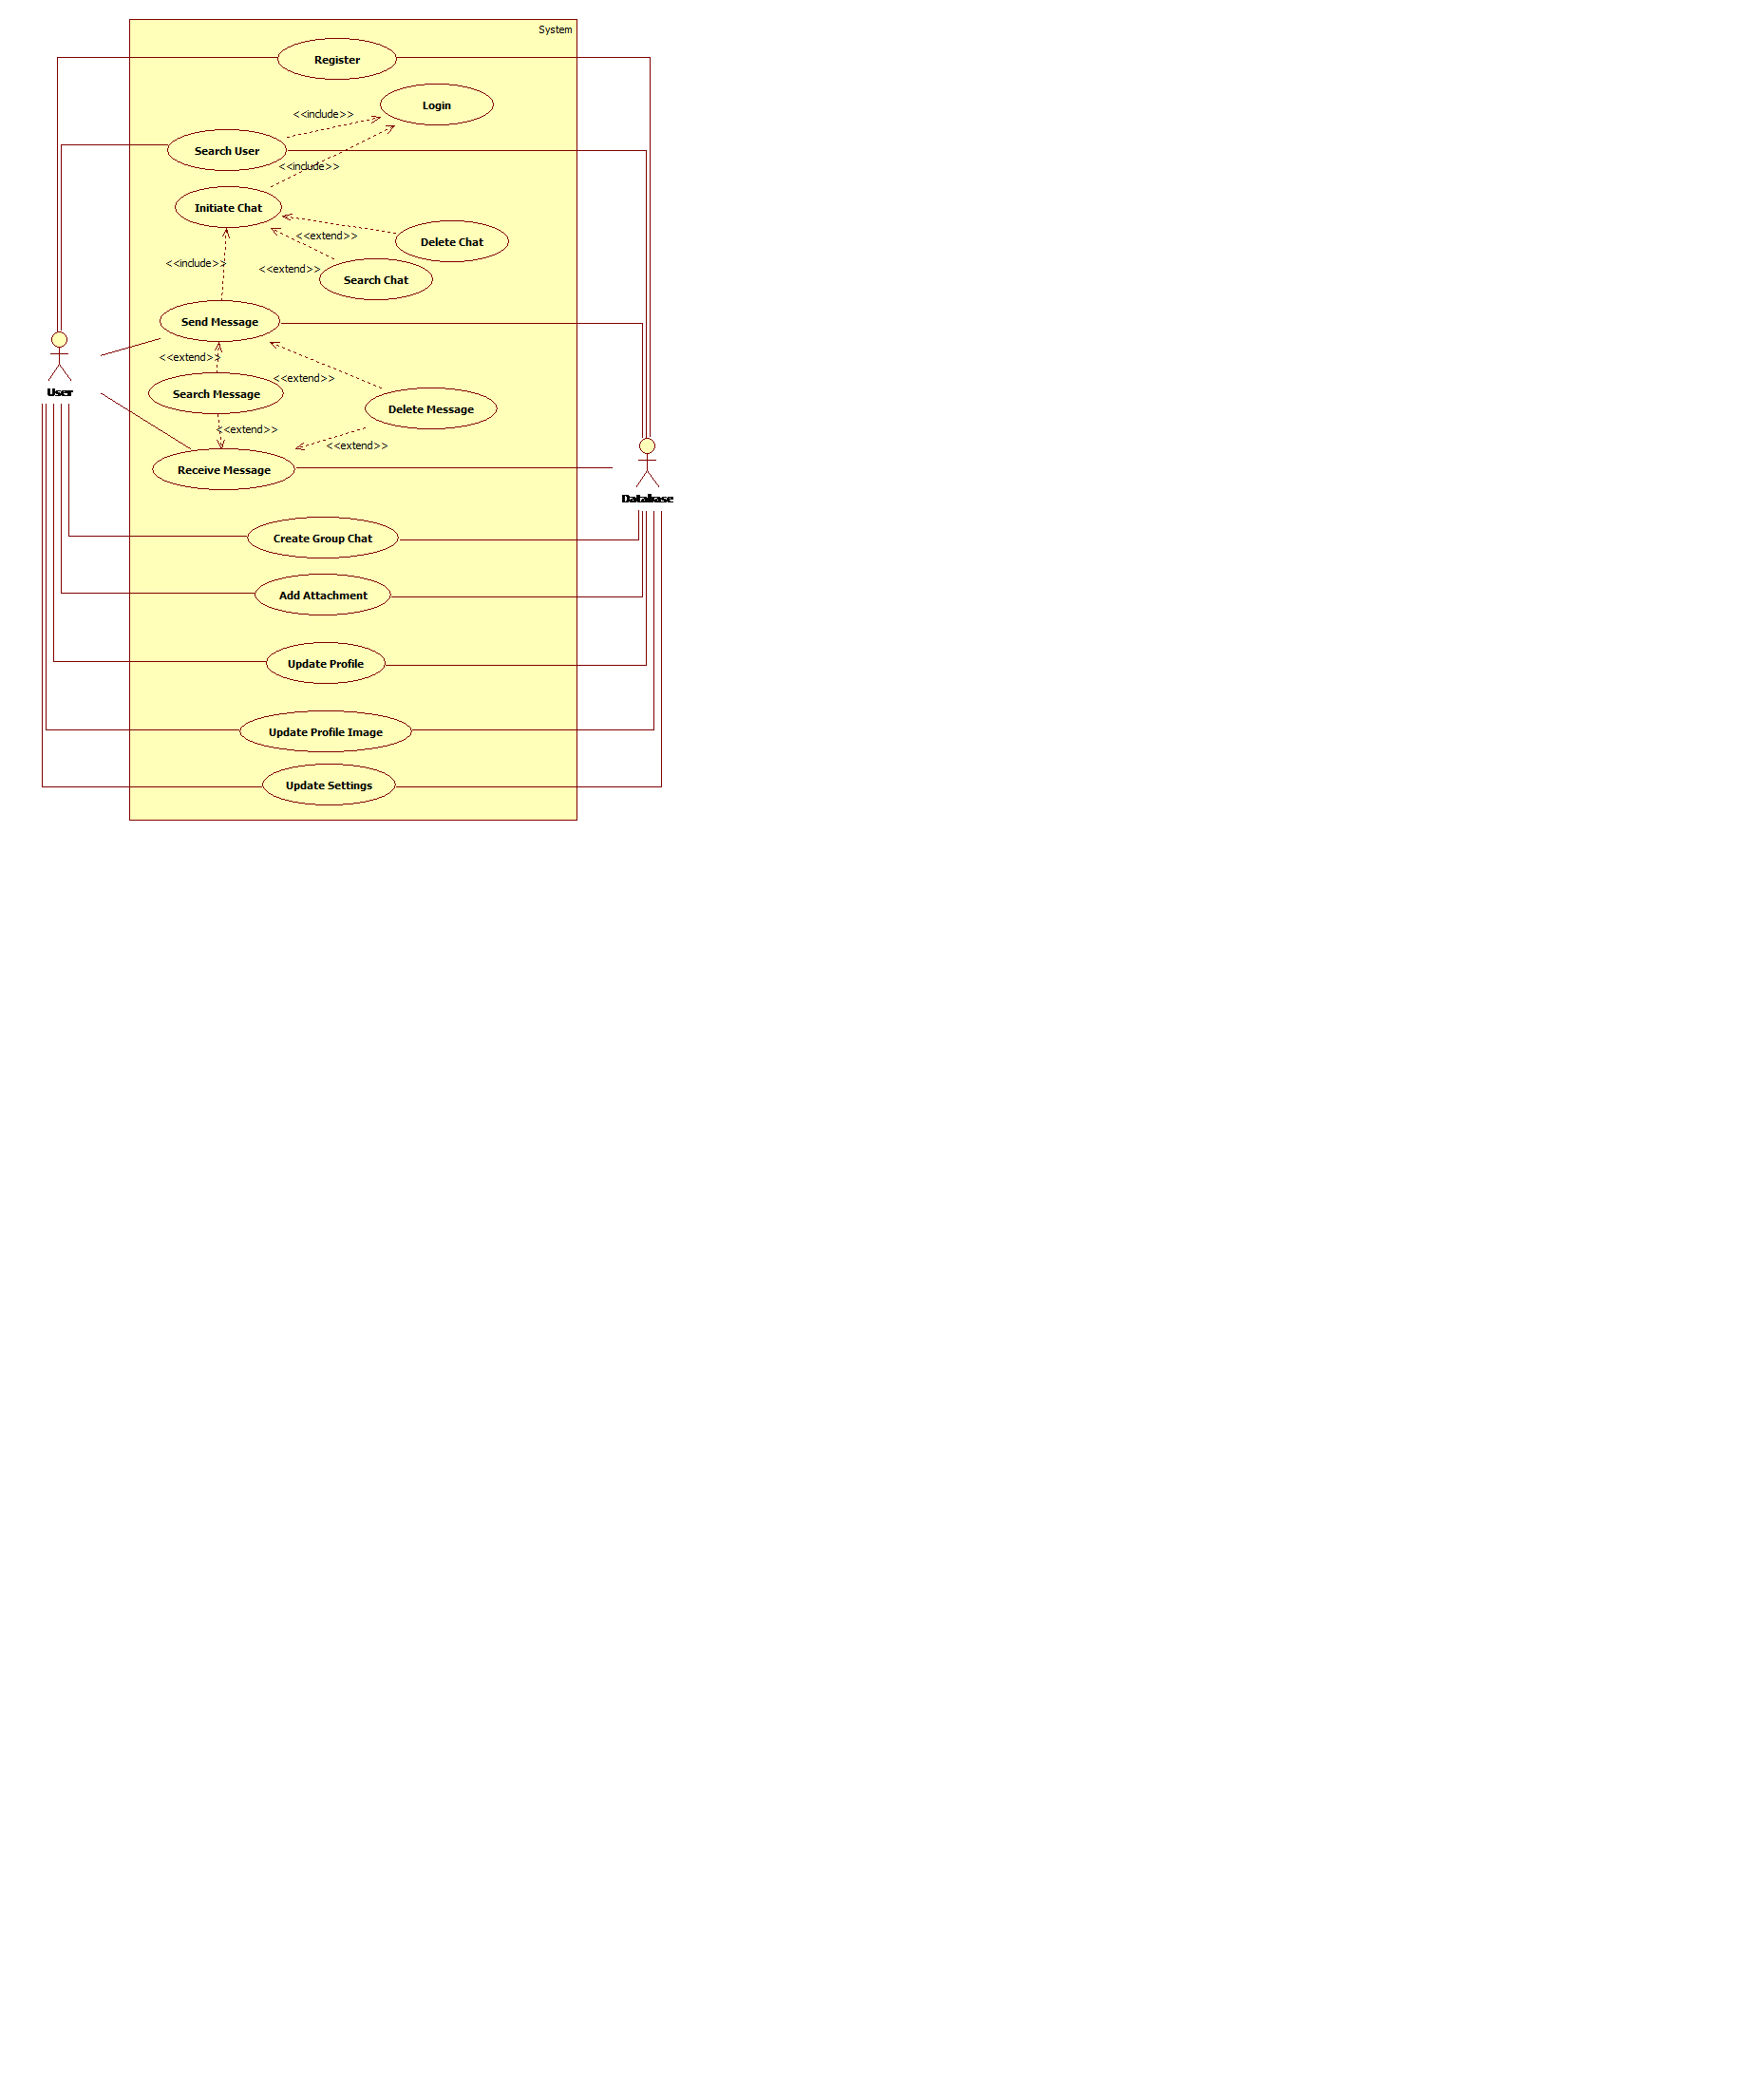
\includegraphics [width=40cm, height=45cm] {useCase_hermes}

\subsection{Functional and Non-Functional Requirements}
\subsubsection{Functional Requirements}
Functional requirements of the system were derived and shown in the use case diagram were then prioritised taken in consideration the time frame given to complete the project and core requirements that the system must at least have such as search user, initiate chat, send and receive messages. Any chat system should have at least these requirements to meet its user’s needs. However, as chat systems have also other features embedded in them and as described in the captured user stories, these requirements were also derived from the user stories but were given a could priority meaning that they will only be implemented after all the core requirements have been implemented and taken into consideration not only the time constraint for this project but also other factors that were identified earlier in this chapter such as strengths and weaknesses of the team. The table below illustrates the prioritisation of these requirements. \par

\begin{center}
\begin{tabular}{ |p{5cm}|p{5cm}|p{5cm}|  }
 \hline
 \multicolumn{3}{|c|}{Core Requirements (requirements that the system must or should at least have)} \\
 \hline
 Functional Requirement ID & Functional Requirement & Description\\
 \hline
 FR1 & Register & The user must be able to sing up to the system from the website or mobile app.\\
 \hline
 FR2 & Log-in  & The user must be able to log-in into the system.\\
 \hline
 FR3 & Search User & The user will be able to search other users. \\
 \hline
 FR4 & Initiate Chat & The user must be able to start chat with other users he/she searched and found. \\
 \hline
 FR5 & Send Message  & The user must be able to send messages once a chat is initiated.\\
 \hline
 FR6 & Receive Message  & The user must be able to receive messages from the other end user.\\
 \hline
 \multicolumn{3}{|c|}{Optional Requirements (requirements that the system could or won't have)} \\
 \hline
 FR7 & Search Chat & The user could be able to search chats they have initiated. \\
 \hline
 FR8 & Search Message & The user could be able to search a message within a chat. \\
 \hline
 FR9 & Delete Chat & The user could be able to delete the entire chat should they wish to do so. \\
 \hline
 FR10 & Delete Message & The user could be able to delete the entire chat. \\
 \hline
 FR11 & Create Group Chat & The user will not be able to create a group chat adding as many users as they wish. \\
 \hline
 FR12 & Add Attachment & The user will not be able to attach a file e.g. pdf, png, etc.\\
 \hline
 FR13 & Update Profile & The user could be able to add or update their status, nick name, etc. \\
 \hline
 FR14 & Upload Profile Image & The user will not be able to upload a profile image to their profile.\\
 \hline
 FR15 & Update Settings & The user could be able to update their settings such as notifications, primary email, etc. \\
 \hline
\end{tabular}
\end{center}

\subsubsection{Non-Functional Requirements}
Non-functional requirements that describe the constraints under which the system should operate are as follows: 
\begin{itemize}
\item The system should be user-friendly and easy to use (usable). 
\item The system should be compatible with all age groups e.g. have a reasonable font-size, colours, etc. 
\item The system should be secure e.g. authentication and/or encryption of passwords and/or messages. 
\item The system should be reliable i.e. it should always work as expected. 
\item The system should be available always e.g. database unavailability can have a huge impact on the system’s availability which will affect its reliability in delivering the service. 
\item The system should have a high performance, high throughput and less latency/delays which all help to increase user’s satisfaction.
\item The system should be transparent i.e. the user does not need to know specific information to use the system. 
\item The system should be able to process user’s messages concurrently e.g. a user’s process should be independent of another user’s process. 
\item The system should be portable e.g. can be used on different portable devices and/or web browsers. 
\item The system should be responsive i.e. process user’s requests as quickly as possible. 
\end{itemize}

\newpage
\section{Modelling and Design}
\subsection{Database Schema}
\subsubsection{Assumptions}
During the conceptual data model, three main entities were identified: ‘User’, ‘Chat’, and ‘Message’. The ‘User’ entity represents data related to each user once they register, it consists of different attributes such as ‘userid’ to uniquely identify each user, ‘username’ that the user sets during registration which is unique for each user, ‘password’ that the user creates for authentication purposes, ‘email’ which the user uses during registration which is also unique and used as the main way of contact e.g. during password reset procedure, ‘name’ which is the user’s actual full name, ‘status’ which is the account’s status to indicate if the account is active (1)  or inactive (0), ‘createDate’ to indicate the date on which the account was created, and ‘modifyDate’ to indicate the date on which the account was modified. \par
The ‘Chat’ entity represents data related to each chat once it is initiated by the user, it consists of different attributes such as ‘chatID’ which uniquely identify each chat, foreign key attributes to uniquely identify the user who initiated the chat, and user with whom the chat is initiated, ‘KeyValue’ for encryption purposes, and ‘CreateDate’ to indicate the date on which the chat was initiated. The entity could have more foreign key attributes if the chat was to include more users e.g. group chat. It could be extended later to satisfy the requirements for a group chat. \par
The ‘Message’ entity represents data related to each message within a chat, it consists of different attributes ‘MessageID’ which is a primary key to uniquely identify the message, foreign key attributes to uniquely identify the chat that the message relates to and the sender of the message, ‘Content’ to store the actual content (text) of the message, and ‘ReceiveDateTime’ to indicate the date on and time at which the message was received. \par

\subsubsection{Entity-Relationship Diagram (ERD)}
An Entity-Relationship Diagram (ERD) was also constructed to represent these entities, their attributes and the associations between them as follows: \newline
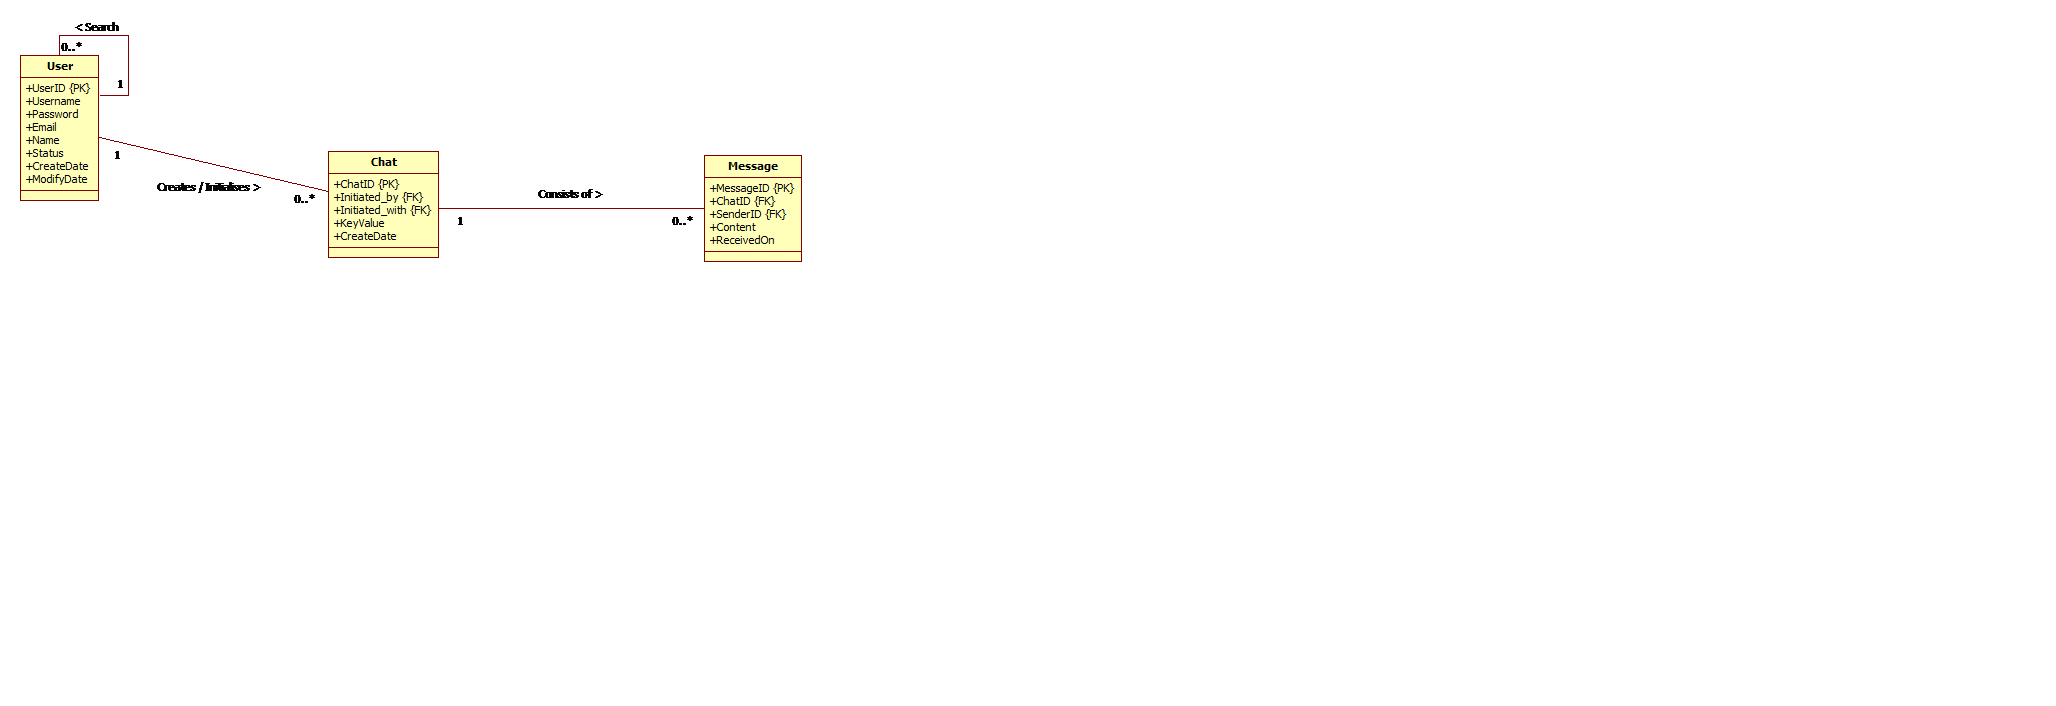
\includegraphics[width=40cm, height=15cm]{erd_hermes}

As shown in the diagram above, a user can search many users but not necessarily all users within the system. In addition, it is possible that the user could have not searched other users yet. A user can initiate zero chats e.g. if they have just recently joined or many chats, each with a different user. Each chat consists of at least one message. \par

\subsection{System Architecture}

\subsubsection{Hardware Architecture}

\begin{itemize}
\item \underline{Machine (i.e. PC or laptop)}: to be able to use some development tools such as GitHub, Notepad++, Android Studio, Android emulator and many more, a machine is needed to develop the proposed software system, compile the code and test it when necessary. 
\item \underline{Smart Phone i.e. Android}: a smart phone which utilises Android as an operating system is also required to test the application from within the device to ensure it is usable and working as expected. 
\item \underline{Web Server}: a web server is also required to store the website’s files, the database including stored procedures and other application’s logic.
\end{itemize}

\subsubsection{Software Architecture}
\begin{itemize}
\item \underline{Android over IOS}: The Android platform was chosen over IOS to develop the phone’s application as it is open source and easily accessible. In addition, other factors had an impact on the decision taken such as familiarity with Android and Java programming language and unfamiliarity or no previous experience with IOS and the time frame for this project was not adequate to learn and develop the system over IOS from scratch.
\item \underline{Java Programming Language}: Familiarity with Java programming language was an advantage as the android application was developed using Java and XML so the time that was supposed to be dedicated to learn Java was instead dedicated to develop the Android application. 
\item \underline{Android Studio}: In the beginning, IntelliJ IDEA was the target Java development environment to use. However, at a later point, Android Studio was launched because it is widely used, specific to Android and empowered by IntelliJ IDEA. In addition, an emulator can be downloaded to test the application from within the IDE so there is no need to run the application on an Android smart phone when testing is required. 
\item \underline{PHP Web Programming Language}: PHP is a server side programming language which is very popular in the development of web applications. Group members are all familiar with the programming language and some of them also have previous experience, this was the main reason why the language was chosen. In addition, PHP supports OOP and MVC, and this can be taken as an opportunity to develop a real-life application using MVC, the most popular and suitable design pattern for development of web applications.
\item \underline{Text or Source Code Editor}: Notepad++ is the chosen editor to be used as it is widely used. However, group members who may be more comfortable at using other editors such as atom should feel free to do so. 
\item \underline{MySQL Database}: Previous knowledge with MySQL among group members, the language suitability of use with Java and web applications, having studied advanced SQL prior to the development of this project were all the main reasons behind the decision to build the database using MySQL. In addition, MySQL is a relational database query language which is suitable to build the database based on the schema previously designed. 
\item \underline{MVC (Model-View-Controller) Design Pattern}: This is a known design pattern that is usually implemented along with Object-Oriented based applications. Its main purpose is to separate the concerns of the application by dividing it into different layers (multiple responsibilities) not only to make it easier to test and maintain but also to make the system components independent of each other so a change in one component would not affect other components. The model represents the persistent data of the application or the business domain i.e. usually entities or classes to represent objects while the view is the actual presentation or layout of the data e.g. web pages. The controller controls and processes user’s tasks. It acts as a consultant to the users and as a mediator or an intermediary point between the model and view. For instance, when the user submits a form, the controller is consulted, the controller then contacts the model which has the persistent data of the application and probably short-live session beans for a user session, and once the request is processed, the controller is notified so that it renders the updates to the user \cite{tutorialspoint}. 

\item \underline{Stored Procedures}:
The database and server-side for this project are cornerstones which will tolerate and respond to all the stress of the software. Also, one of the most important quality factors of software is consistency which could be affected by server design and behaviour with the database. For fulfilling both parts, we decided to use stored procedures which provide some main benefits as follows: \par
\begin{itemize}
\item There will be only one change when making a change in interactions with the system which could be costly and time consuming.
\item Having the same operation with the data and storing the data into the database which will guarantee consistency and integrity of the data in our database.
\item In an event when some validation is required to be applied, this can be done once at the server side, instead of doing it separately on each platform which may cause errors and redundancies. 
\item Less time consuming as there will be no redundancy in the implementation and also supports the maintainability and re-usability of the system.
\item Increases security remarkably because it will encapsulate the queries inside the database and no third party will be able access or amend them.
\end{itemize}
\end{itemize}

\subsection{System Prototypes}
Prototypes for both platforms were designed using PowerPoint to aid in the implementation of a clean GUI. They can be found in Appendix A (Web App: section A.1, Android App: section A.2). 

\newpage
\section{Implementation}
\subsection{Methodology and Framework}
\subsubsection{Agile Development}
In contrast to traditional software development processes which are plan-based, the agile process focuses on simplicity and divide and conquer manner of problem-solving. Accordingly, will provide a system that fulfils customer's needs. The Agile development consists of different methods such as XP and Scrum \cite{Agile-Scrum}. More infromation about Agile and the Agile principles can be found in appendix B, section B.1. 

\subsubsection{Scrum: Sprints}
The Hermes project was designed and developed based on Scrum framework in an attempt to meet specific user requirements in a short time by increasing productivity to allow earlier delivery of deliver-ables. Most of the sprints will fit into a two weeks’ time frame which will all together result in a final working version of the system. A detailed plan of the iterations of this project can be found in appendix B, section B.2. 

\subsection{GUI Implementation}
\subsubsection{Android App GUI}
The implementation of graphical user interface in java is quite straight forward. The interfaces are designed using XML (Extensible Markup Language) with the help of widgets such as Buttons, Image Views, etc. These can be directly designed in Android Studio with a simple drag and drop interface or via XML code. We used both the methods as per our requirements.
Some third-party libraries were also included for special interaction functionalities. The swipe a chat to delete interface was provided by a library call SwipeMenuListView \cite{lib2}. It is a simple list view with the added functionality of handling options when swiped. The delete Chat functionality was implemented with the help of this. Colour Palettes were used to make enhance the GUI \cite{ColorHex}. 
Another library was used for implementing emojis as seen in WhatsApp and Facebook Messenger. This was called “emojicon” and is publicly available on GitHub \cite{lib1}.
One thing to notice here is that the XML and Java parts of the application are very intricately linked to each other. Thats why all the libraries used for user interface are also used in Java (Activities) for updating and manipulation of the interface elements. 

\subsubsection{Web App GUI}
In Hermes-website GUI is implemented by using HTML5 and CSS3.
In Hermes HTML5 is written straight on the IDE without using any library or and other remote link. We are using HTML5 because   HTML5 is the newest version of HTML. It introduces simplified tags, new semantic and media elements, and relies on a set of JavaScript libraries that enable web applications and also CSS is the style standard for HTML5 many people include CSS when they use the term “HTML5” to describe the family of technologies used to create web applications.
HTML5’s new elements are a superset of HTML 4 elements, which means older pages will continue to work in modern browsers. HTML5 introduces elements that add new semantics to your pages, giving you more options for creating web page structure than we had with HTML 4.01.
WHY CSS? So as to get complete control on the presentation of pages, often without even changing your XHTML.
\begin{lstlisting}
<link rel="stylesheet" type="text/css" href="css/main.css" />
<link rel="stylesheet" type="text/css" href="css/login_signup.css" />
\end{lstlisting}

\subsection{Application Structure using MVC Design Pattern}
\subsubsection{Android Application}
The system has been implemented following the MVC design meaning that the code can be segregated into model, view and controller classes based on their functionality.\par
The view part of this approach consists of the user interface that is required for interaction of the application with the user. Fortunately, Android has its own language to develop the user interface known as XML (Extensible Markup Language). It is a very simple markup language like HTML but with more widgets for better user interaction. Thus, we don't need additional styling language like CSS in case of HTML. At the back-end, this view is linked to an android activity (constructed using the Java language). This activity controls the touch events and updating the view or user interface. It can thus be used to perform specific tasks at each transition of the life cycle. For example, if we get a call while using our application, the activity pauses, so we can stop all the processing and network related tasks until the activity resumes. \par
The model is a form of local volatile data storage for the application. It stores all the important data as class objects that is required by the application during its execution. All the data is lost when the application shuts down. For example, A chat information class is used to store all important data about a chat like chatID, user IDs of the sender and receiver, etc. This data can then be manipulated and displayed during the run time of the application. Our android application has models for chats, users and messages to aid in the implementation of the use cases. \par
The controller is responsible for managing the data between the view’s activity and the model and the database. It takes data from content providers like the databases and stores them in the model. It then displays this data to the view for user interaction. In our android app, we have created a controller that works in the background to obtain the data. This controller has no direct link to the view’s activity and thus cannot directly update the view. An interface was thus created to facilitate the update of views from the controller and to delegate control to the user activity. It is as follows -
\begin{lstlisting}
public interface AsyncResponse {
    public void processfinish(ArrayList<ChatInfo> output);
}
\end{lstlisting}
This controller uses this interface to delegate control to a view’s activity by passing an array list of ChatInfo objects (which is the model for chats). Similar is the case for handling messages and users.

\subsubsection{Web Application}
The website is implemented primarily by using “JAVASCRIPT” and more precisely by using “AJAX” technology to make it more dynamic.
\begin{lstlisting}
var xhr = new XMLHttpRequest();
xhr.open("POST", "../php_files/" + page, true);
xhr.setRequestHeader("content-type", "application/x-www-form-urlencoded");
xhr.send(data);
\end{lstlisting}
In this system JAVASCRIPT is implemented by following the MVC Design so as to reduce the user’s interaction with the core requirements and make system robust and also to achieve isolation so as to keep each function/feature isolated from other feature so we can prevent other features from failure if some or any feature(s) fails.
controller.login() - > model.callAjax() -> redirect to home or view.responseMessage() // for failure
User is interacted only with the controller portion of this website.
JSON data format is used instead of Xml or CSV to transfer  and receive information from JAVASCRIPT to PHP
\begin{lstlisting}
str = JSON.stringify({"chatId":"0",friendId: 
friendId,"message": msg}); // sending data to php
$jsonstr=json_encode($arr);// receiving data from php
return $jsonstr;

\end{lstlisting}

PHP is only used to interact with the data base and to deliver the pre-defined pages .“No use of cookies” policy is implemented to increase the security. Sessions are used to keep track and flow of information on server side. 
\begin{lstlisting}

session_start();
$_SESSION[ 'username' ] = $username;
$_SESSION[ 'name' ] = $arr[ 0 ][ 'Name' ];
$_SESSION[ 'user_id' ] = $arr[ 0 ][ 'UserID' ];
\end{lstlisting}

To interact with the database instead of using PHP pre functions, PDO Class is used. The biggest advantage of using it as we can easily switch between databases of different organizations. 
\begin{lstlisting}
$user="id865672_admin";
$pass="Admin";
try{
  $pdo= new PDO('mysql:host=localhost;dbname=id865672_hermesdb',
  $user, $pass);   }
 catch(PDOException $e){print "Error!:" . $e->getMessage() . "<br/>";
 die();} 
 
\end{lstlisting}

\subsection{Core Implementation}
\subsubsection{Android Application}
The core functionalities include login, sign-up, search for a user, initiate chat, send and receive messages. All these tasks have one thing in common that is, in all these functionalities, the application needs to connect with the server to interact with the database. But network operations put a drain on resources and we do not want the application to seem laggy and hang. So, we used AsyncTask class of Java to perform the network operation like sending and receiving data from the server and database. The AsyncTask class performs an operation in a separate thread from the GUI and asynchronously. Its format is like this - 
\begin{lstlisting}
    class GetChats extends AsyncTask<String, Void, String> {

        public AsyncResponse delegate = null;
        @Override
        protected String doInBackground( String[] userID) {
            // TODO Auto-generated method stub

            final StringBuilder builder = new StringBuilder();
            //Do Your stuff here..

            final HttpClient httpclient = new DefaultHttpClient();
            final HttpPost httppost = 
            new HttpPost("http://hermes.webutu.com/ChatSelect.php");

            final HttpGet httpget = 
            new HttpGet("http://hermes.webutu.com
            /SP/ChatSelectUserAll.php?userIDV="+
            String.valueOf(userID[0]));
            String result;
            HttpResponse httpresponse = null;
            ArrayList<NameValuePair> postParameters;
            postParameters = new 
            ArrayList<NameValuePair>();
            postParameters.add(
                    new BasicNameValuePair("userID", 
                    String.valueOf(userID[0])));
            try {
                httppost.setEntity(new 
                UrlEncodedFormEntity(postParameters));
                // reset to null before making a new post if it's being reused
                httpresponse = null;
                httpresponse = httpclient.execute(httpget);
            } catch (IOException e1) {
                e1.printStackTrace();
            }

            if(httpresponse!=null){

                try {

                    // Get the data in the entity
                    BufferedReader reader = new BufferedReader(
                    new InputStreamReader(
                    httpresponse.getEntity().getContent(), "UTF-8")
                    );


                    for (String line = null; (line = 
                    reader.readLine()) != null;) {
                        builder.append(line).append("\n");
                    }
                } catch (IOException e) {
                    e.printStackTrace();
                }
            }
            return builder.toString();
        }
        @Override
        protected void onPostExecute(String result) {
            super.onPostExecute(result);
            //chats.clear();
            chats = new ArrayList<>();

            JSONObject finaljson = null;
            try {
                JSONArray jArray = new JSONArray(result);
                finaljson = jArray.getJSONObject(0);

                Log.v("JSON OUTPUT: ", finaljson.toString());

                for (int i = 0; i < jArray.length(); i++) {
                    try {
                        JSONObject oneObject = jArray.getJSONObject(i);
                        // Pulling items from the array
                        chats.add(new 									
                        ChatInfo(oneObject.getInt("fk_InitUserID_by"), 				
                        oneObject.getInt("fk_InitUserID_with"), 					
                        oneObject.getInt("ChatID"), 							
                        oneObject.getString("Username"), 						
                        oneObject.getString("Name")));
                    } catch (JSONException e) {
                        // Oops
                        e.printStackTrace();
                    }
                }
            }catch (JSONException e) {
                e.printStackTrace();
            }
            delegate.processfinish(chats);
            //this method will be running on UI thread
        }
\end{lstlisting}

In this code block, we also see multiple other things at work. For instance, the HTTP POST functionality is included so that it can be used in the future instead of HTTP GET. Moreover, the response received from the server is in JSON format. It has to be parsed to extract the actual data. This is done using the JSONArray and JSONObject classes of JAVA as shown above.
This AsyncTask class is located in all the controllers of each model of user, chat and messages. In the one shown above, a user’s information about all his/her chats is extracted from the database and stored in the model ChatInfo class and an array of these ChatInfo Objects is passed to the GUI for user interaction.
Here, we also understand why a controller cannot directly interact with the view because the GUI is on one thread and the controller is running on another thread and thus needs an interface in between to delegate control. All the main functionalities were implemented using the same approach. For login and signup, the passwords were hashed even when storing them in the database. \par
Software development on android is based on JAVA which is an object-oriented language and thus our application is developed using OOP approach.
The Integrated Development Environment (IDE) Android Studio has been of immense help and it really aided in timely completion of this application. The inbuilt debugger and logcat were very instrumental in finding bugs.


\subsubsection{Web Application}
The index.php page of the hermes-website  is the entry point for all other pages contained in the website.Through this page user is allowed to access three main features namely “LOGIN”,”SIGNUP” and “GET STARTED”. This page is completely implemented by HTML5 for structuring and CSS3 for presentation. Each feature, “LOGIN”,”SIGNUP” and “GET STARTED” has its specific structure so specific page is dedicated  to each feature which has the path as follows. \par
\begin{lstlisting}
Root/php_files/login.php,
Root/php_files/signup.php
Root/php_files/get_started.php. 
\end{lstlisting}
Although each feature has its own page but none of them can be accessed directly. Each page is fetched by using  JAVASCRIPT (“AJAX” technology) MVC Design. 
JAVASCRIPT only updates a specific portion of the page not the entire page which results in reducing the overloading of the network and also reduce the size of response data.
On loading the main page We set  onclick event on all the buttons on the page. \par
\begin{lstlisting}
window.onload = function () {
document.getElementById("login_page").onclick 
= controller.main_buttons;
document.getElementById("signup_page").onclick 
= controller.main_buttons;
document.getElementById("get_started_button").onclick 
= controller.main_buttons;
};
When user click on Login button 
(<a href="#" id="login_page" class="link">Login</a>) . 
JAVASCRIPT call the "controller.main_buttons" event handler
var controller = {
main_buttons: function (event) {
event.preventDefault();
		var target = event.target;
		var id = target.id;
		model.pageCall(id);
	}
}
That fetch the id of the clicked button and transfer it to 
"model.pageCAll(id)" which is an AJAX call

var model = {
	pageCall: function (data) {
			view.loader();
			var xhr = new XMLHttpRequest();
			xhr.open("POST", "php_files/" + data + ".php", true);
		xhr.setRequestHeader("content-type",
		"application/x-www-form-urlencoded");
			xhr.send(null);
			xhr.onreadystatechange = function () {
if (xhr.readyState === 4) {
if ((xhr.status >= 200 && xhr.status < 300) 
|| xhr.status === 304) {
		var response = xhr.responseText;
		view.responseData(data, response)
				}
}	
			};
		}  
\end{lstlisting}

When the model get the data, it sends response and corresponding id to view.
responseData(data, response) which displays the requested data on the browser and sets the onclick event on the submit buttons of responded data. \par
\begin{lstlisting}
responseData: function (data, response) {
document.getElementById("main_div").innerHTML 
=response; 
if (data === "login_page") {
document.getElementById("login_submit").onclick 
= controller.login;
} else if (data === "signup_page") {
document.getElementById("signup_submit").onclick = 
controller.signupValidation;
} else {
document.getElementById("loader").innerHTML 
= "<h2 class=\"warning\">Failed To load Data </h2>";

     }
	},
<\end{lstlisting}
And again the cycle restart for the new submit button rendered on the page and controller.login() - > model.callAjax() -> redirect to home or view.responseMessage() // for failure 
Note: If the response coming from the PHP code which is connected to the database that response received from the server is in JSON format.It has to be parsed to extract the actual data and then send to the view.\par
\begin{lstlisting}
arr = JSON.parse(xhr.responseText);
\end{lstlisting}
In the home page, timers are used to make AJAX call again and again to update the specific potion of the page.  
Examples for contacts list updating and chat updating are as follows: \par
\begin{lstlisting}
setInterval(controller.latestChat, 4000);
setTimeout(function () {model.loadData(data, "loadChat", 
"load_data.php");}, 2000);
\end{lstlisting}
We used onKeyUp event to activate search username call from the database and to enter messages in the database to get rid of clicking the submit button. \par
\begin{lstlisting}
document.getElementById("search_box").onkeyup = controller.searchUser;
document.getElementById("message_box").onkeyup = controller.writeMessage;
\end{lstlisting}


\subsection{Implementation of Security Features}
\subsubsection{Android Application}
The application uses hashing techniques for the sensitive user data like passwords. 
For maximum security, we are using SHA-256 algorithm for hashing. 
The following function is used to generate hash code for a string -
\begin{lstlisting}
      public byte[] getHash(String password) {
        MessageDigest digest=null;
        try {
            digest = MessageDigest.getInstance("SHA-256");
        } catch (NoSuchAlgorithmException e) {
            // TODO Auto-generated catch block
            e.printStackTrace();
        }
        digest.reset();
        return digest.digest(password.getBytes());
    }
\end{lstlisting}
This function returns a binary hash value and we convert it into hexadecimal for easy storage in the database. This is done using bin2hex function as shown below-
\begin{lstlisting}
         static String bin2hex(byte[] data) {
        	return String.format("%0" + (data.length*2) + 
        	"X", 	new BigInteger(1, data));
    		}
\end{lstlisting}
Right now,the application uses HTTP GET requests to interact with the server but we have implemented the ability in our code to change it later to HTTP POST whenever the server is ready for extended security. 

\subsubsection{Web Application}
We prevent our user information by not storing the password as Plain text. Instead we used hashing technique to encrypt the password.SHA-256 algorithm was used for hashing passwords and to further extend the security, we used HTTP POST requests to deliver or receive the data from the server.
\begin{lstlisting}
$p=hash("Sha256",$password);
\end{lstlisting}

\subsection{Software Testing}
The time constraint and unfamiliarity with JUnit and unit testing in PHP were the reasons for not performing unit testing on the implemented system so debugging was instead used to reveal errors and correct them. However, the system was functionally tested during the implementation to ensure that the system works as expected. Structural testing was not considered as the system is not critical and performing such kind of testing would be costly. Functional testing is widely used and helps to test the functional requirements of the system. Functional tests were performed to test the correctness of the system, any unsuccessful tests were repeated until successful and they can be found in Appendix C. \par
It is important to mention that usability tests were performed to ensure the system is fairly usable. Acceptance testing could not be performed as this kind of testing requires real users and data and the system's behaviour cannot be known when it is used by real users. 

\newpage
\section{Team Work}
Immediately after forming a team, we have created a group chat on WhatsApp to easily communicate with each other. We also used to make video and audio calls to each other when necessary. Facebook messenger was also used to communicate with each other e.g. when a group member cannot reach us on WhatsApp for some reason. We have had a couple of meetings to discuss the specifications and requirements and we also used to communicate via email. It was hard for all of us to use GitHub in the beginning but later after considering some online documents and watching some tutorials we got used to using it. Some group members had difficulty using it but we made sure to guide and help them. \par 
In the beginning, after forming a team, we started the initial plan. Khalil and Arsalan worked on the initial plan. The problem was clearly understood, and the aims and objectives were clearly defined. A decision was made on which methodology and framework to follow to manage and control this project and deliver it on time. Similar systems such as web and android applications were also examined to better comprehend the design and technical aspects of such systems. During the initial plan, we have also identified the system’s primary and secondary actors, captured a set of user stories (scenarios) to better understand how the user would like to use the system and derive the functional requirements which will be as accurate as possible. The requirements were prioritised taking in consideration the time frame given to complete this project and other factors using MoSCoW (Must, Should, Could, Won’t) \par
We also used UML notation to construct a use case diagram to define the system’s actors and their requirements. An entity relationship diagram was also constructed during the conceptual data model to represent our database schema. We have also come up with a set of non-functional requirements to define the constraints under which the system will operate. These deliverables were produced during our meetings on and off campus. Power Point was also used to design the wireframe prototypes for both the web and the android applications to make the implementation chapter for us as developers smoother. We then started working on the web and android applications, Khalil and Arsalan had several meetings with Vashu to guide him build a web application using MVC OOP. They also started working on the Android application after launching Android Studio and we also took responsibility to help Vashu work on the web application. \par
We then created a LaTeX project as specified to share the documentation with the other group members. Communication and collaboration is very important in team projects and since Yatharth was away for a couple of weeks and Vashu was not communicating and collaborating as well as he should have been, this had an impact on the initial plan of the project which could be identified from the ambiguity in the project organisation (the second section of the initial report). Vashu informed us that he was going abroad three days before the initial report submission which of course adversely impacted the initial plan even though he managed to finally produce the work he was assigned within these three days just before the submission and the presentation. This has also affected the overall implementation and productivity. \par
When Yatharth returned, and joined the team, he was instructed as appropriate so he can catch up with the group. He dedicated the required time and showed commitments and responsibility working on the android application along with Khalil and Arsalan which has accelerated the development of the android app. \par
Upon receiving the feedback on the initial report and despite the issues we had, we had several meetings to discuss our progress. We worked side by side to produce a marking schema that all group members will eventually agree on. The schema seemed to satisfy all the group members and we eventually had an agreement. Khalil and Arsalan’s responsibilities were to work on the Android and web applications, database including stored procedures, and the documentation while Vashu’s responsibility was to work on the web application and Yatharth’s responsibility was to work on the Android application. A strict policy was produced and signed by all group members which included the terms and conditions and the marking schema to minimise the risks and any future failures. \par
We decided to review the initial plan to determine if we should re-prioritise our requirements taking in considerations the issues occurred and potential risks. We have used a technique named as SWOT analysis to identify the internal and external factors that may have an impact on our project’s objectives. Additionally, we have identified some potential risks that may arise as we progress and set mitigation and contingency plans to be able to manage and control these risks and most importantly minimise or eliminate them if possible. \par
After multiple discussions, we decided to sign up to a web hosting company to implement our database using MySQL and since it provides an interface called phpMyAdmin and allows us to access our files through FileZilla, modify them and apply any updates immediately, we believe that this tool was necessary as it allows group members to remotely access the files and the database from their local machines and also test the files when necessary and particularly the web app unlike GitHub (the code cannot be run remotely on there). \par
In the policy signed by all members, we agreed to develop both platforms using the MVC design pattern, object-oriented approach, and use the same centralised stored procedures for both the web and the android applications to maintain the integrity and consistency of the system and to avoid redundant implementation. Even though Vashu agreed on using MVC OOP, and SPs in the beginning, he disagreed later even though we taught him about the MVC design pattern, its use, the object-oriented approach i.e. classes in php and magic getters and setters, and the purpose of using SPs. At this stage, a conflict has occurred because of the disagreement which of course delayed the development process of the web application. \par
Therefore, we decided to create a new website as a compensation which was going to be MVC OOP and to use the same centralised stored procedures on the server because we could not take the risk. We then realised that creating a new web application is time consuming and can be riskier so the only option to avoid the risk was to carry on with the web application we already have built and re-configure it to work with the same server side. \par
Since then, we started to have regular meetings twice or more per week. Vashu started communicating and attending our meetings, and carried on working on the web application with the help of all group members who made sure the web application uses the same SPs as the android one and is synchronised to work with it. Khalil and Arsalan worked on all parts of documentation throughout the project while the other members helped with the implementation chapter. Validation and verification were used to examine that both applications are working correctly and to check the applications against its specifications and user’s requirements. Therefore, functional testing was performed. \par
Group meetings were the most effective in terms of working together, communicating and collaborating and producing individual and group tasks based on the responsibilities assigned to each group member. Email and WhatsApp were the most effective tools to communicate and keep group members updated throughout this project. In addition, productivity tools such as GitHub and LaTeX were also effective to accelerate the development process, share the documentation and share the workload among group members. Other tools such as UML, and FileZilla were less effective in terms of facilitating group work but the fact that they were helpful and effective in the construction of the system cannot be denied. \par
In conclusion, despite of the conflicts and issues we had, we still have worked together as a team, developed and delivered both web and android applications. Not only that we have delivered the project on time but also, we improved our communication and collaboration skills and we learned how to work and what to expect from working in a professional environment. In addition, lessons learnt from the conflicts occurred, and we learned how to avoid or tackle such conflicts in the future. 

\newpage
\section{Evaluation}
\subsection{Achievements relative to the plan}
All the core requirements set during the planning phase were successfully implemented with the required quality. In addition, some of the important optional requirements were also implemented meaning the functionality and usability of the system was enhanced further. The system was implemented over two different platforms as stated in the specifications and both the web and android applications were delivered on time. Therefore, primary aims were met and the secondary aims were not fully met. The system has been developed in a manner to easily accommodate the implementation of optional requirements and enable future extensions. Even though, there were certain conflicts and constraints involved during the engineering of the system, we were able to accomplish our objectives to meet our aims. 
\subsection{Limitations and Weaknesses}
\begin{itemize}
\item The design of the Android application GUI is not consistent across different screens.
\item Activities, sequence and class diagrams were not constructed to better define the architecture of the system which could be a weakness in the design phase and could have impacted the implementation of the system. 
\item The Android application does not work without an active Internet connection unlike similar existing systems as the time was not sufficient to implement a local database.
\item The notifications for both platforms could not be implemented as it requires an additional component between the database and the client and we did not have previous experience in that field. 
\item The messages being transmitted are not secured because end-to-end encryption was not implemented. This puts the contents of users' messages at risk of being revealed if the system is attacked. 
\item The applications take a while to load the chats and the messages because all the data associated with a user is being downloaded from the sever periodically. 
\item The Android application uses emojis to provide users with more flexibility to communicate with each other while the web application does not have the same feature because there was no third party library that we were aware of. 
\item The user cannot update his/her details entered during the registration e.g. a change in the email address cannot be made within the system meaning that an updated contact method of the user may be missed. 
\item The user can initiate a chat with any user on the system just by searching a random username and the other end user does not have the option to accept starting a chat or blocking the user initiated the chat which can be a privacy issue. 
\item There is no functionality to save the username or the contact without actually initiating a chat. 
\item User is not informed whether a message is sent, delivered to, received or seen by the other end user. 
\item Unit testing was not performed throughout the implementation phase which could assure a better quality and reveal errors that may have not been revealed. 
\item Libraries and external services which the applications interact with may not be up to date meaning the system may not have optimal performance and embedded features like the existing chat systems.
\end{itemize}
\subsection{Team Work and Personnel Reflection}
Group chat, and email were the primary means of communications which we used to keep each other updated. Group meetings on and off campus were instrumental for performing group as well as individual tasks. Responsibilities were appropriately distributed among team members according to previous experience and familiarity which helped not only accelerated the development of the system but also assured the quality. Each group member was also comfortable working on the their assigned responsibilities which has increased the motivation and productivity. \par

As mentioned in the team work section, a conflict occurred as a team member was not communicating as well as he should have been but later the conflict was resolved and an agreement was reached between all members to deliver the system on two different platforms communicating with one server side to maintain consistent implementation. The occurrence of the conflict taught us a great lesson that we learned and most importantly we learned how to deal with such conflicts. A successful team is a team where all members share the workload, have respect for the project and their colleagues. Despite of the conflicts and issues we had, we managed to work together and overcome the conflicts by appreciating each other' work, helping and motivating each other. The conflict turned to be an advantage to the team as a whole because following the resolve of the conflict, the level of communication and collaboration was significantly increased and all members became more efficient and had more commitments. We think that this has aided in a successful outcome of this project. \par

One important factor which we believe had impacted our team and the project as whole is the less number of members compared to the other teams. In real software engineering projects, a team consists of a number of members such as the project manager, analyst, developers, testers and quality assurance. If we had more team members, the execution of the project's life cycle stages could have been a lot better and in particular the execution of the implementation and testing phases. 
\subsection{Future Work}
\begin{itemize}
\item Enhance the GUI of the android application by making the screens consistent and user-friendly. 
\item Add the notification feature so that the user is notified when a message is received without having to open the app and check. 
\item Implement offline functionality for Android by caching the on-line database into a local database. 
\item Implement end-to-end encryption of messages to secure the system. 
\item Implement a functionality so that the user will be informed of messages being sent, delivered and seen. 
\item Implement the optional requirements to make the system as usable as other existing chat systems like Whats App. 
\item Perform a comprehensive unit testing and also usability and acceptance testing. 
\item Make the web application portable so users will be able to use it on their preferred portable devices. 
\item Re-configure the system to be scalable so additional components can be added and the system will adapt to changes in technology and resources over time. 
\end{itemize}

\subsection{Conclusion}
Working on the group project has been a great experience for all of us. We learned the major software engineering skills such as requirements engineering, software architecture and design, implementation and testing and what to expect and how to perform in a professional software engineering environment. \par
We also learned the importance of working in a team in general and of communication and collaboration in particular. In conclusion, we have become more familiar with the execution of the software life cycle stages and developing software projects from requirements engineering to testing and evaluation. This project was an opportunity to be prepated to put these skills into practice and has inspired us to develop similar systems and further improve skills already acquired in future projects. 


\newpage
\section{Peer Assessment}
\begin{tabular}{| c | c | c | c |} 
 \hline
 Member Name  & Member ID & Mark (Out of 100) & Mark (Out of 25) \\ [0.5ex] 
 \hline\hline
 Khalil Jabir & 1678724 & 104 & 26\\
 \hline
 Arsalan Ardeshiri & 1678493 & 104  & 26 \\
 \hline
 Yatharth Ranjan & 1661609 & 102 & 25.5\\
 \hline
 Vashu Tyagi & 1663661 & 90 & 22.5 \\
\hline
\end{tabular}


\newpage
\begin{thebibliography}{12}
\bibitem{CodeDodle} 
CodeDodle, 2015. Facebook Like Chat Application in PHP. [online] Available at: \texttt{<http://www.codedodle.com/2014/04/facebook-like-chat-applicati
on-in-php.html>} [Accessed 01 February 2017].
\bibitem{ColorHex} 
color-hex, 2017. Popular Color Palettes. [online] Available at: \texttt{< http://www.color-hex.com/color-palettes/popular.php >} [Accessed 12 March 2017]. 
\bibitem{Agile-Scrum} 
Emeraldinsight, 2010. Understanding agile project management methods using Scrum. [pdf] Emeraldinsight. Available at: \texttt{<http://www.gbd.dk/files/649\_{}Understanding\_{}agile.pdf>} [Accessed 13 February 2017].
\bibitem{eStreamChat} 
eStreamChat, 2017. eStreamChat – online web chat software. [online] Available at: \texttt{<http://www.estreamchat.com/>} [Accessed 02 February 2017]. 
\bibitem{DS-Concepts} 
Miles, S., 2017. Concept and Characteristics, 7CCSMDSM Distributed Systems. King’s College London, unpublished.
\bibitem{FB-Messenger} 
Percona Live, 2014. Facebook. [pdf] Percona Live. Available at: \texttt{<https://www.percona.com/live/mysql-conference-2014/sites/default
/files/slides/Percona\%{}20Live\%{}202014.pdf>} [Accessed 01 February 2017]. 
\bibitem{lib1} 
Sachdeva, A., 2015. emojicon. [android library] GitHub. Available at: \texttt{< https://github.com/ankushsachdeva/emojicon >} [Accessed 13 March 2017]. 
\bibitem{SWOT} 
Smartsheet, 2017. SWOT Analysis. [online] Available at:\texttt{<https://www.smartsheet.com/14-free-swot-analysis-templates>}
[Accessed 06 February 2017].
\bibitem{tutorialspoint} 
Tutorialspoint, 2017. MVC Framework - Introduction. [online] Available at: \texttt{<https://www.tutorialspoint.com/mvc\_{}framework
/mvc\_{}framework\_{}introduction.htm>} [Accessed 12 March 2017].
\bibitem{WhatsApp1} 
WhatsApp, 2016. WhatsApp Encryption Overview. [pdf] WhatsApp. Available at: \texttt{< https://www.whatsapp.com/security/WhatsApp-Security-Whitepaper.pdf >} [Accessed 03 February 2017]. \bibitem{WhatsApp2} 
WhatsApp Inc., 2017. WhatsApp Messenger (2.16.396). [android application] Play Store. Available at: \texttt{<https://play.google.com/store/apps/details?id=com.whatsapp
\#{}details-reviews>} [Accessed 02 February 2017]. 
\bibitem{WhatsApp3} 
WhatsApp Inc., 2017. WhatsApp Web. [online] Available at: \texttt{< https://web.whatsapp.com/ >} [Accessed 02 February 2017]. 
\bibitem{lib2} 
Zhang, B., 2016. SwipeMenuListView. [android library] GitHub. Available at: \texttt{< https://github.com/baoyongzhang/SwipeMenuListView >} [Accessed 13 March 2017]. 
\end{thebibliography}

\newpage
\begin{appendices}
\appendix
\section{System Prototypes}
\subsection{Web Application Prototype}
\begin{center}
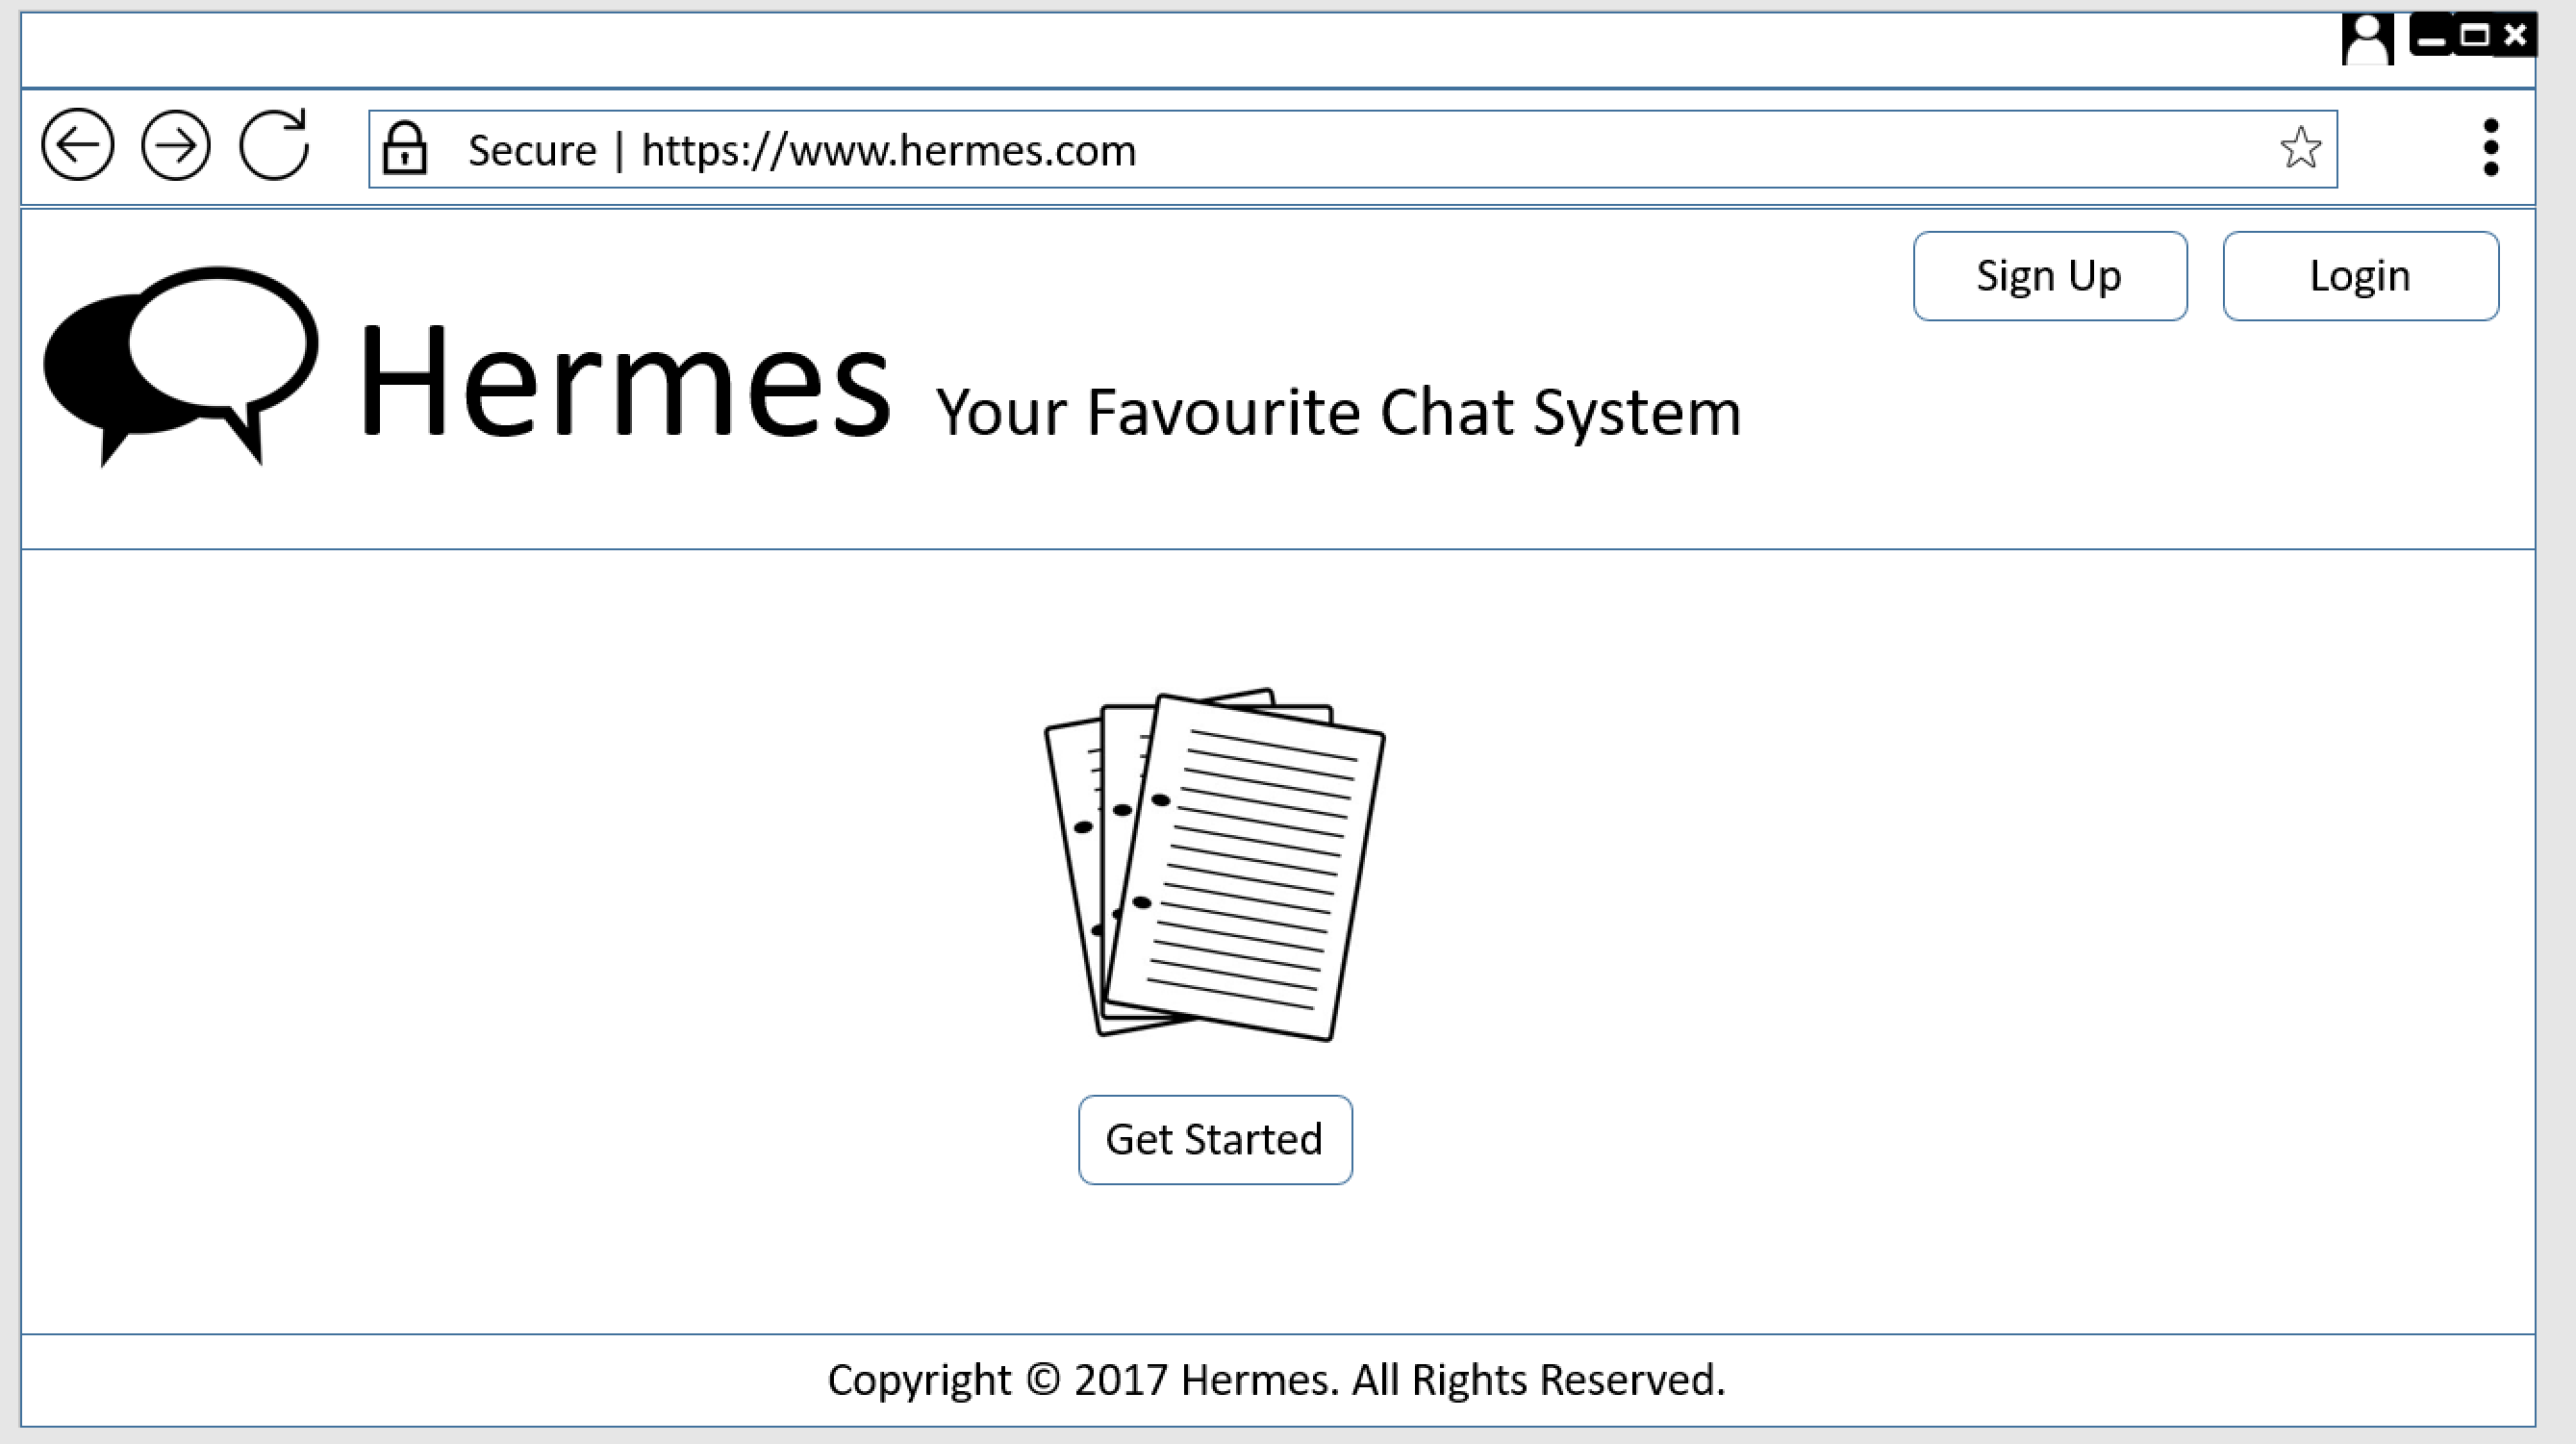
\includegraphics[width=10cm, height=5cm]{w1}
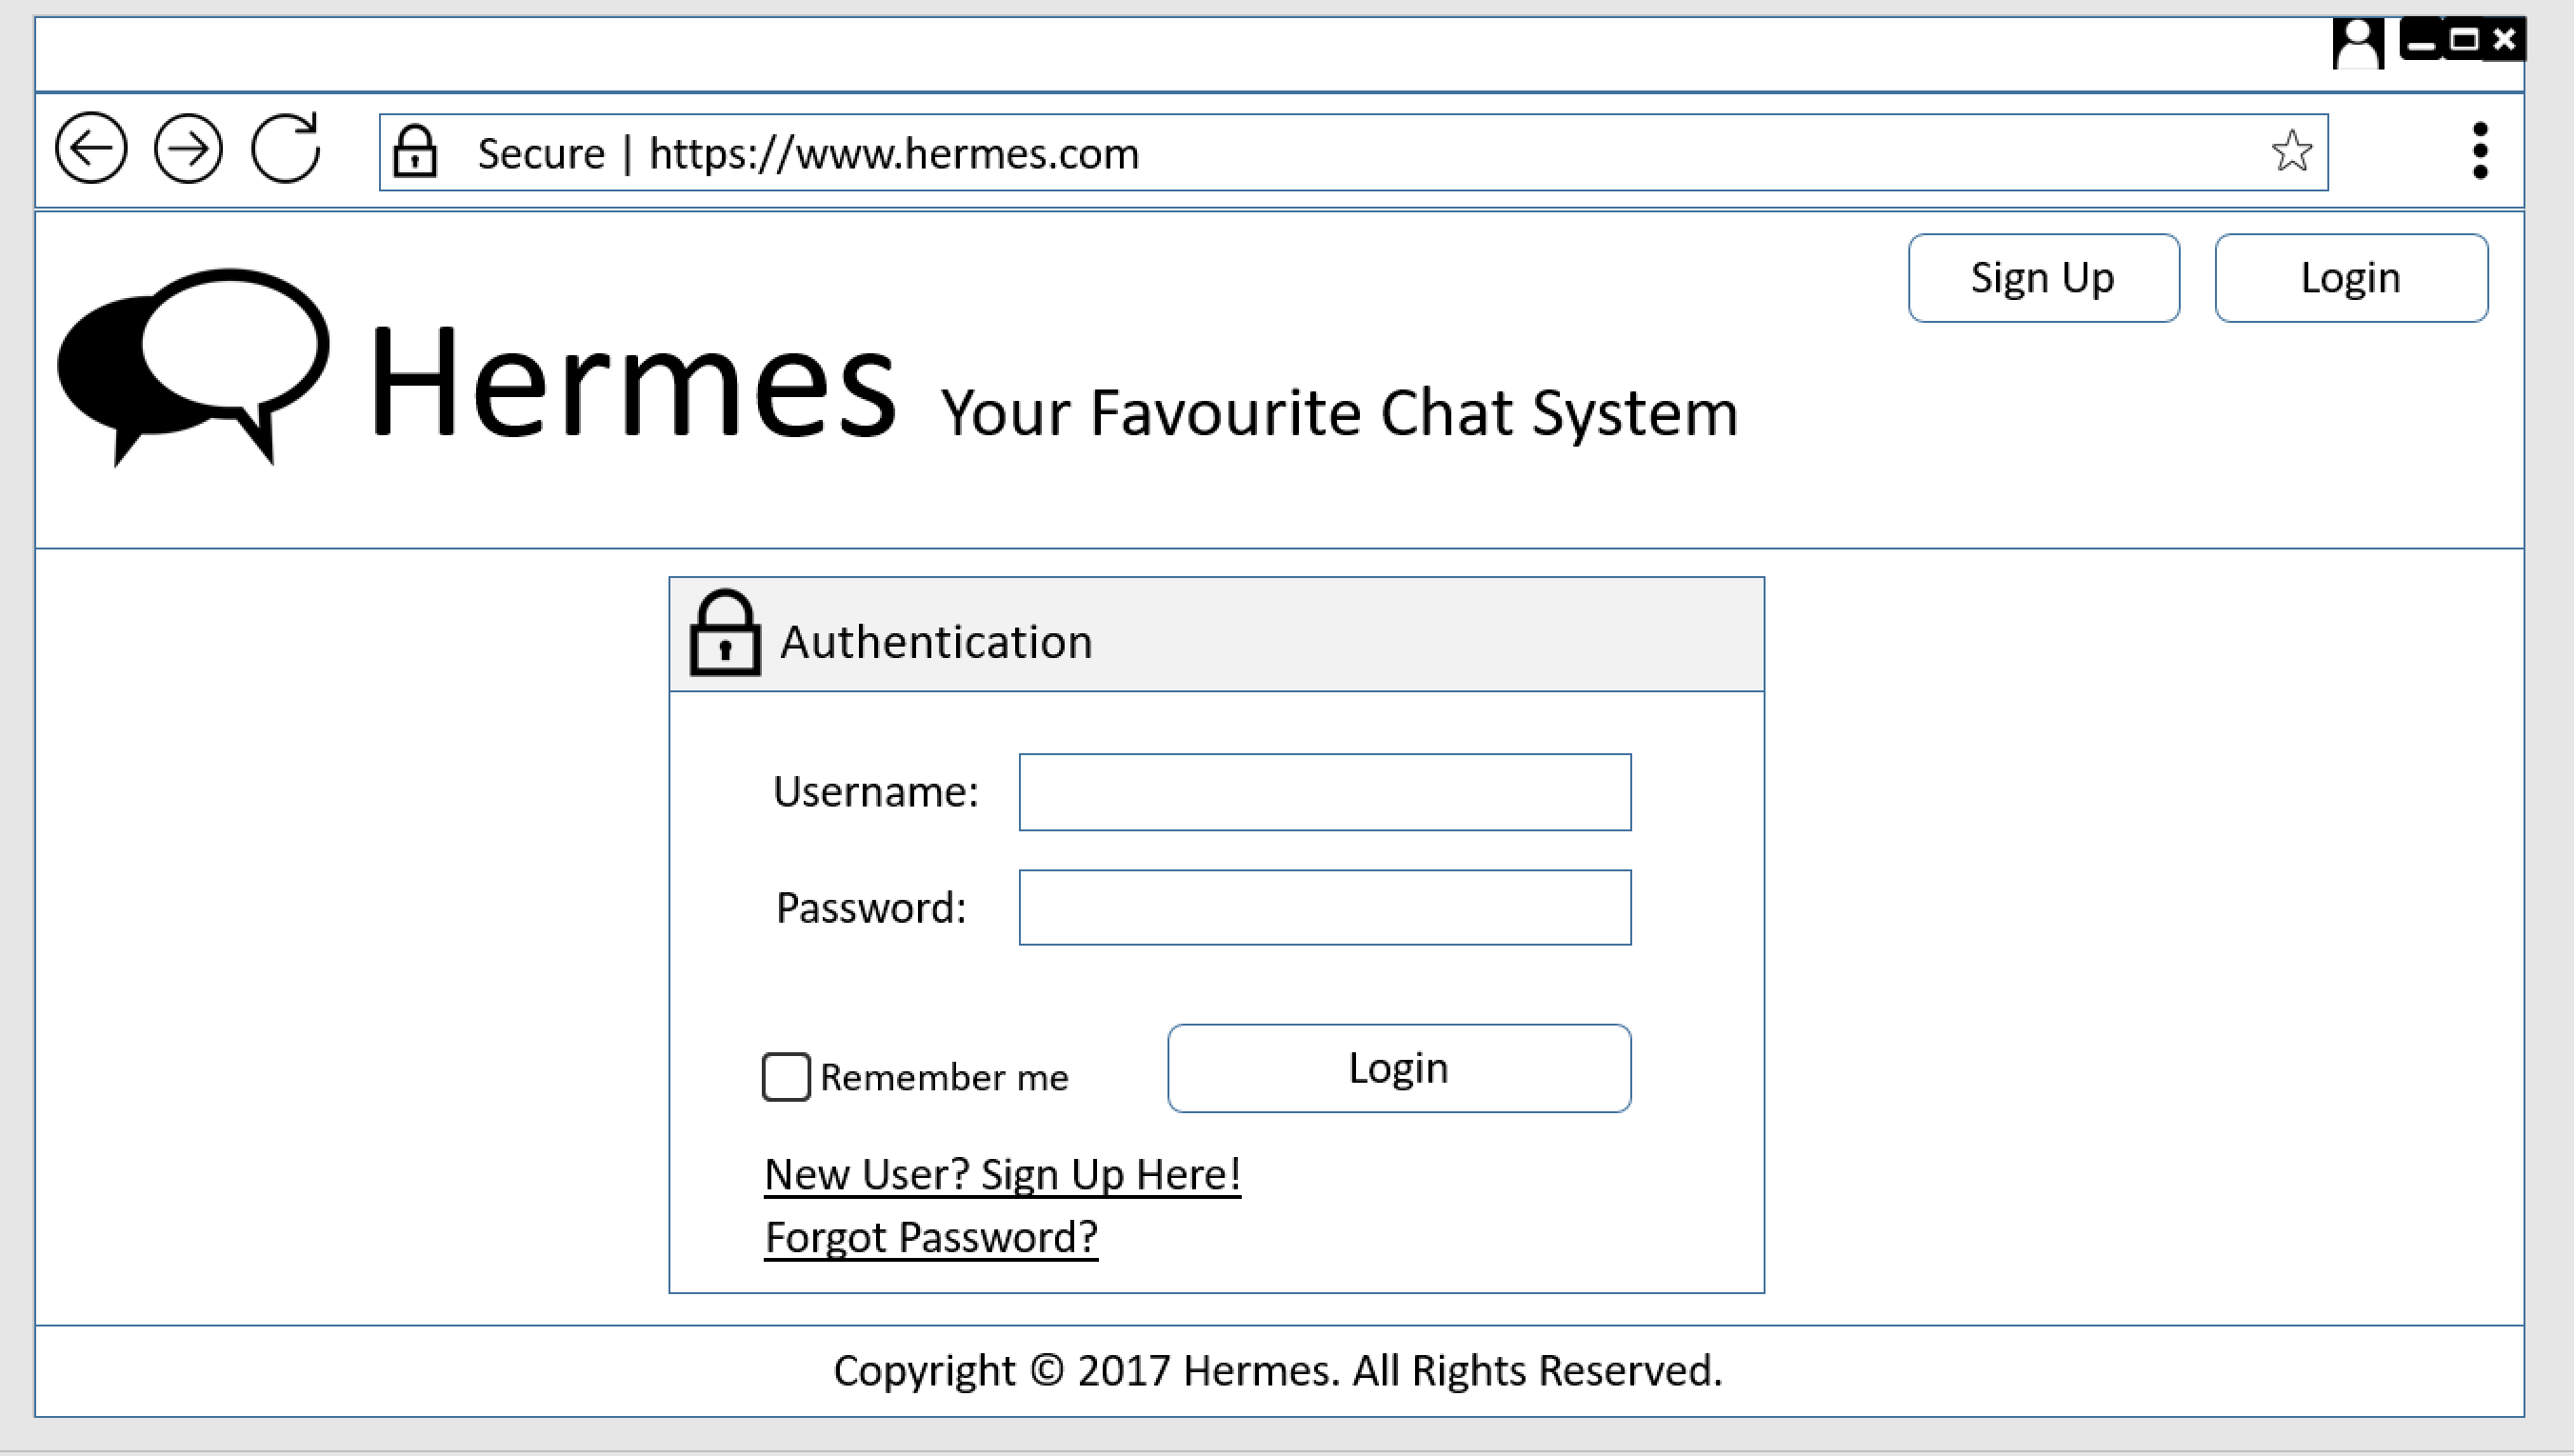
\includegraphics[width=10cm, height=5cm]{w2}
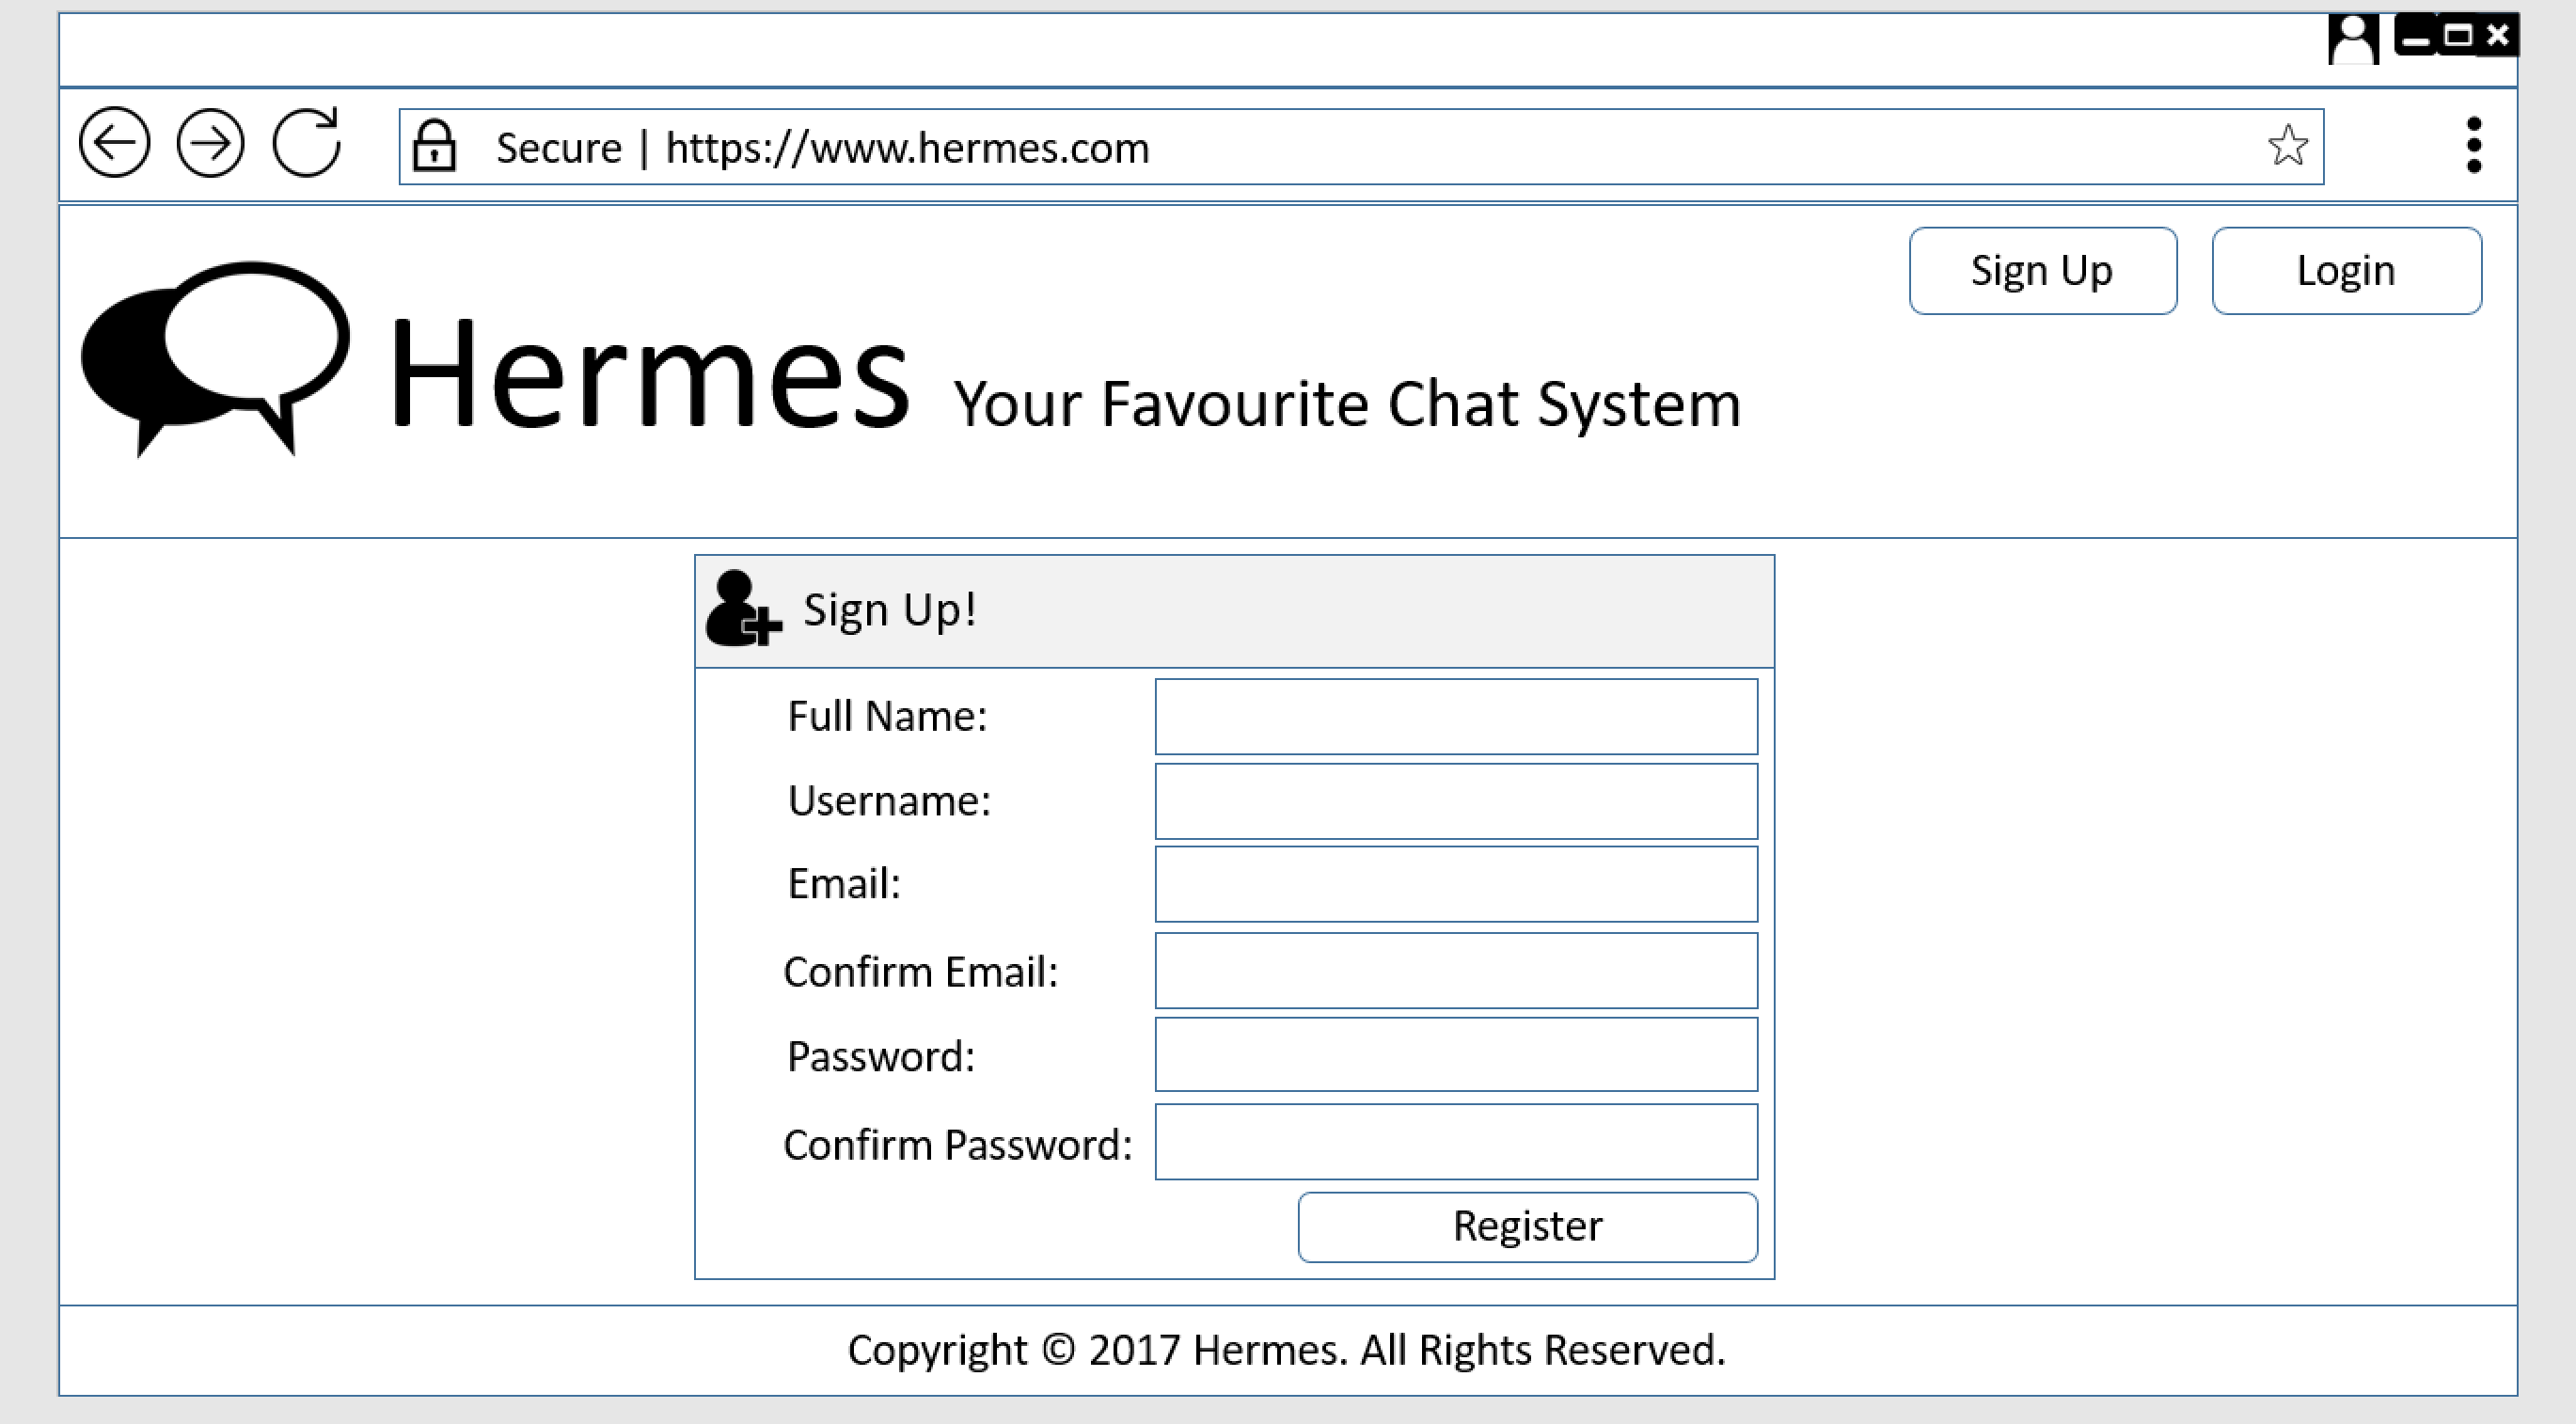
\includegraphics[width=10cm, height=5cm]{w3}
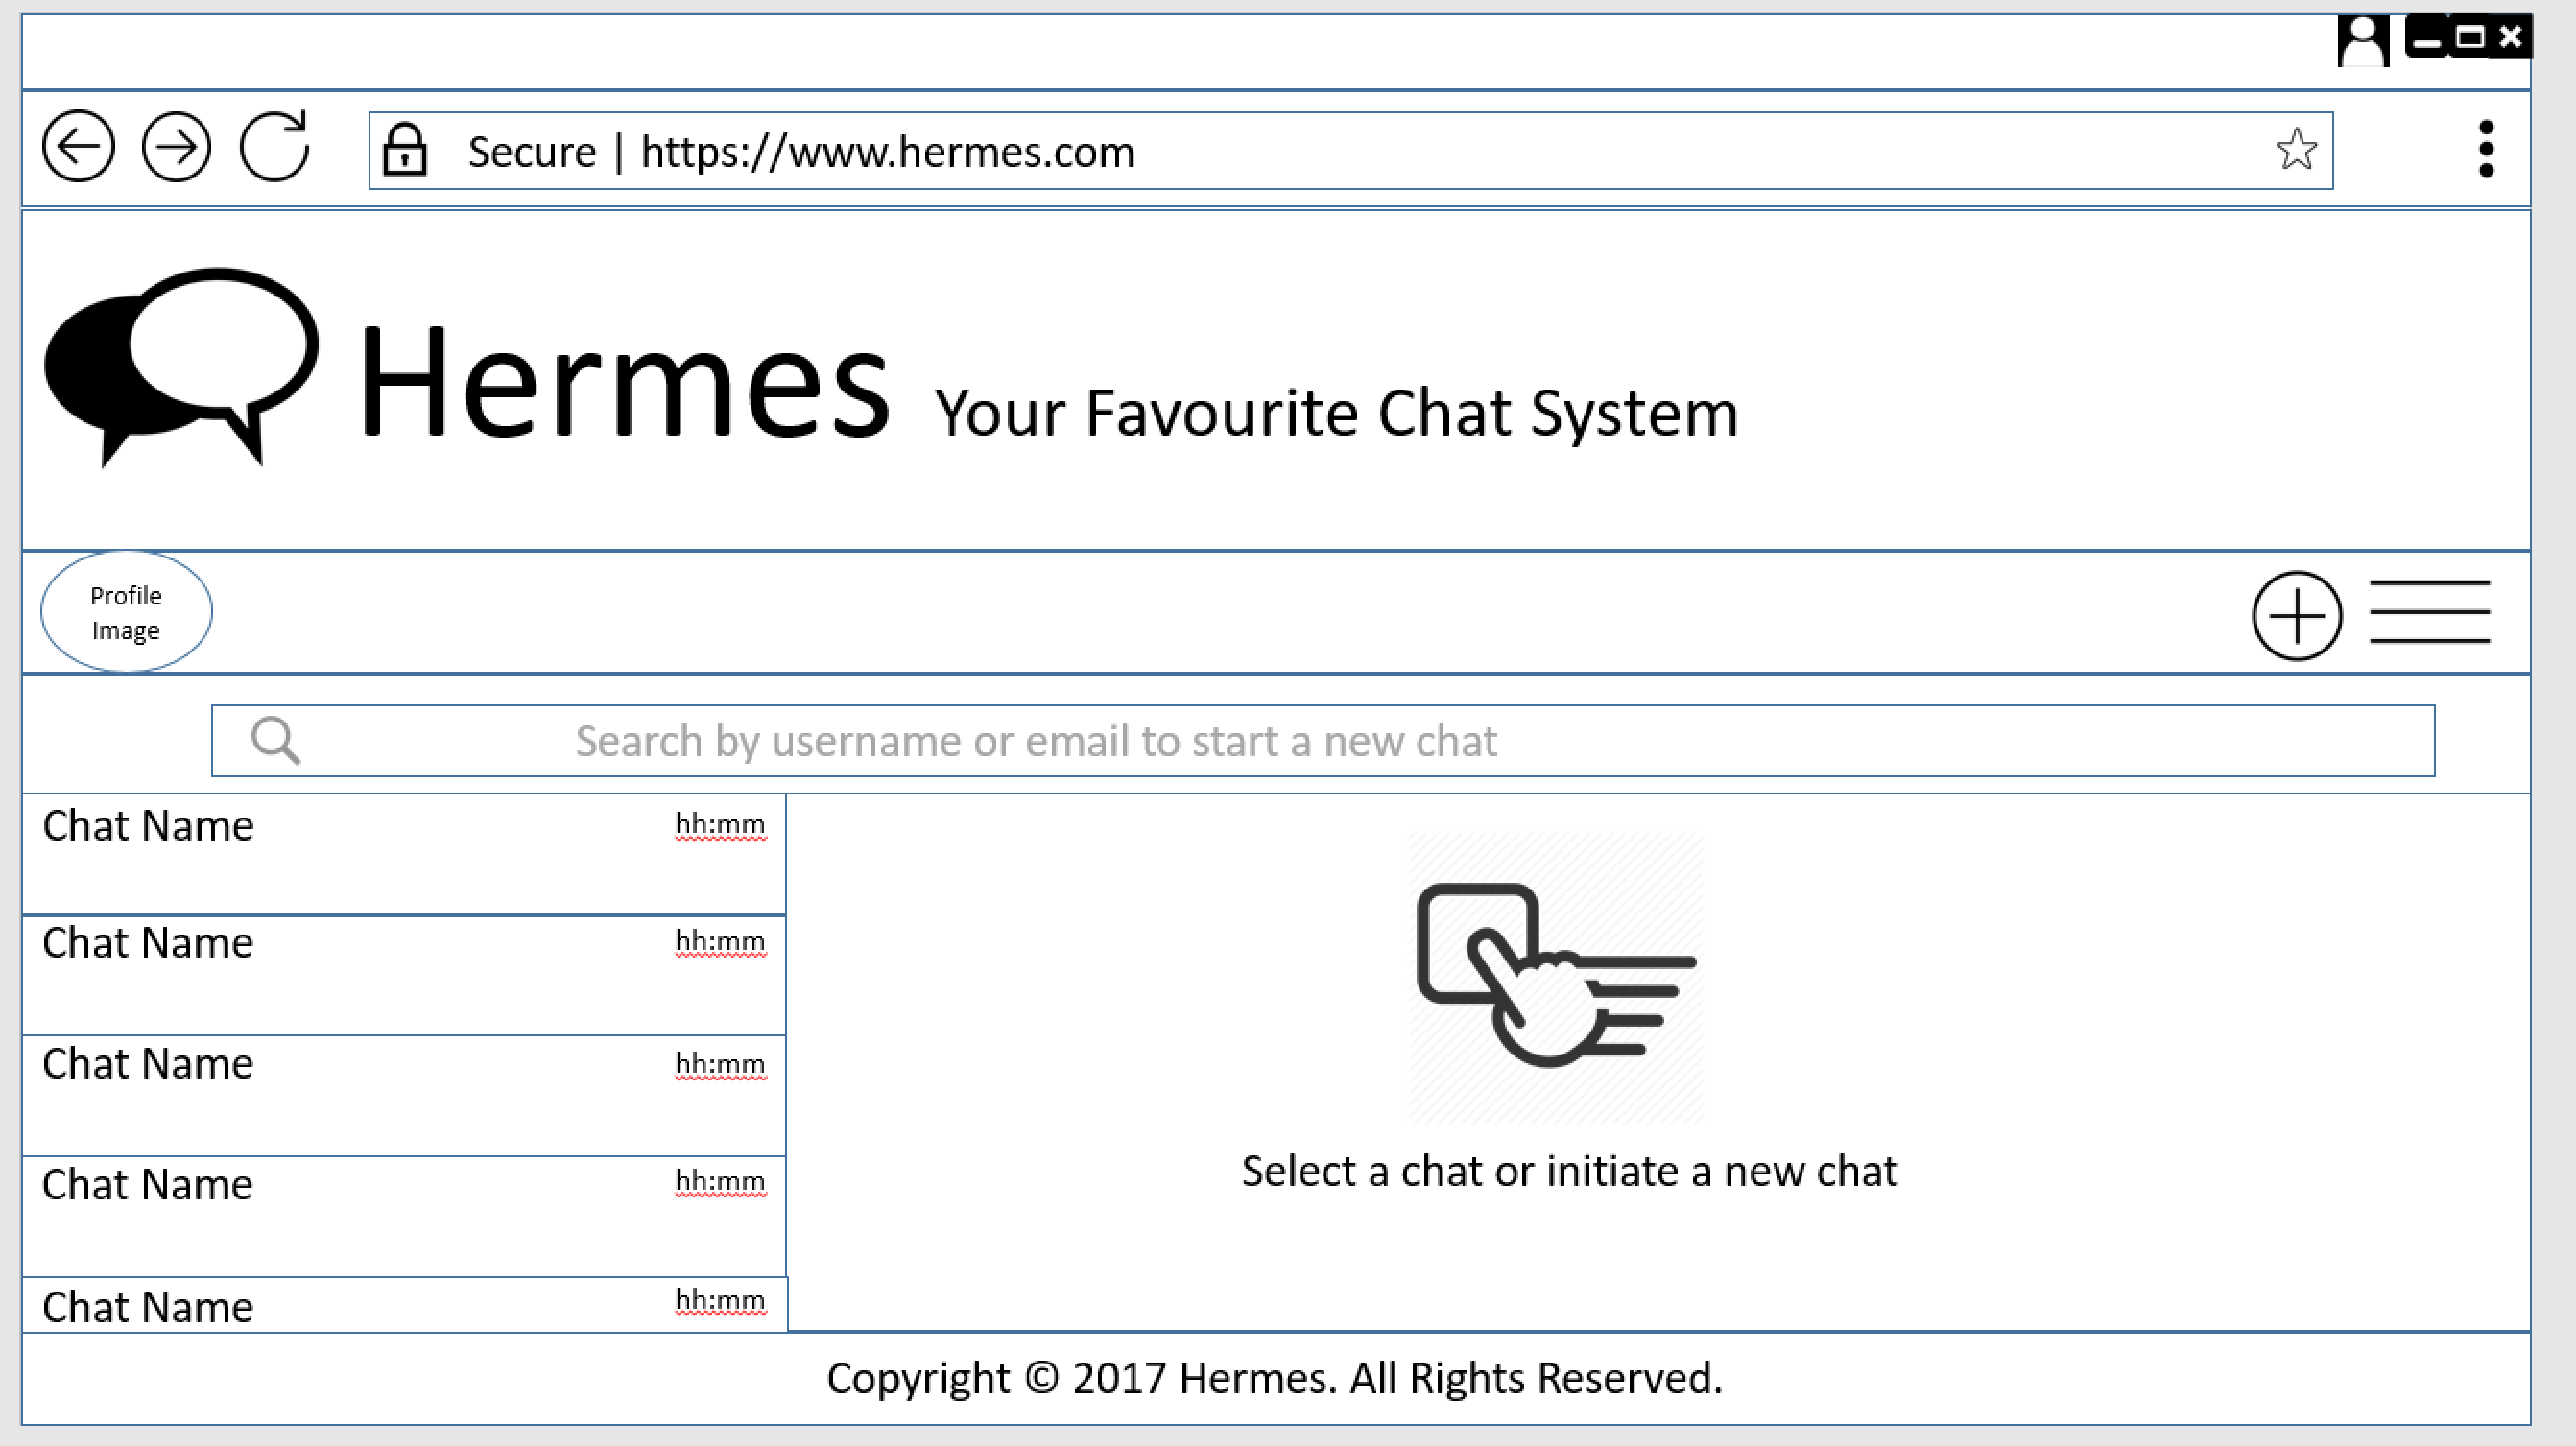
\includegraphics[width=10cm, height=5cm]{w4}
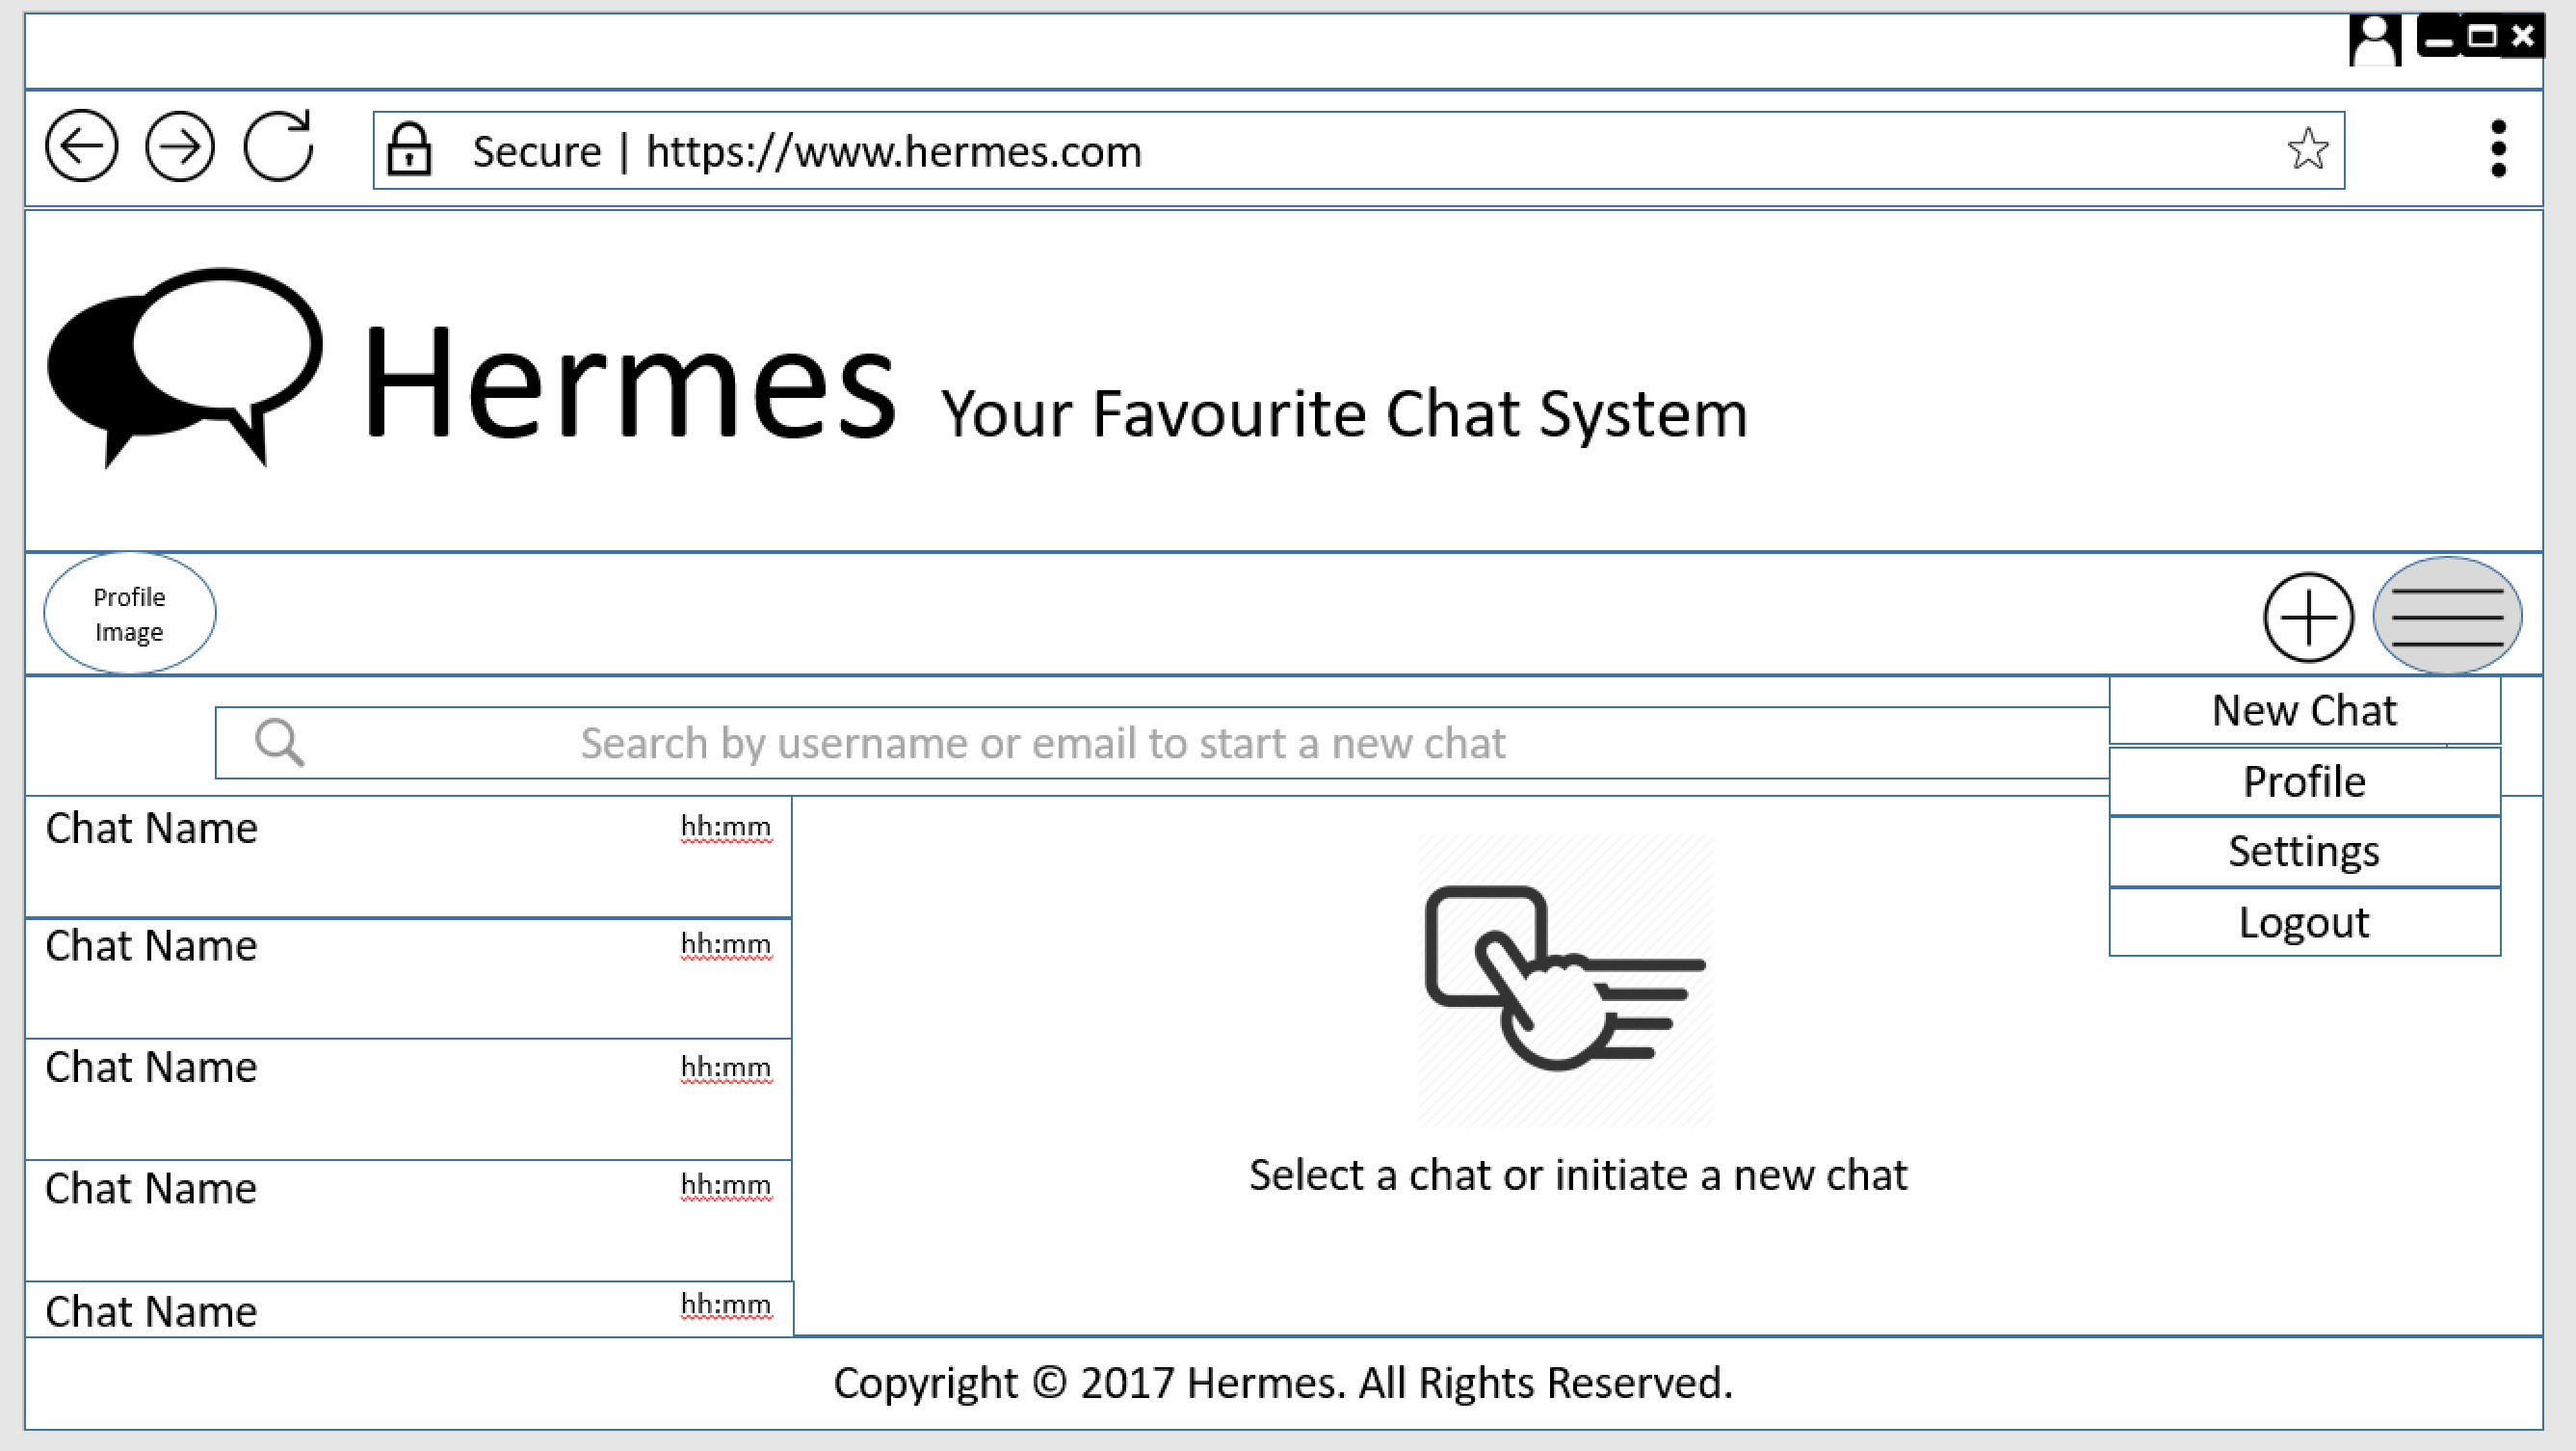
\includegraphics[width=10cm, height=5cm]{w5}
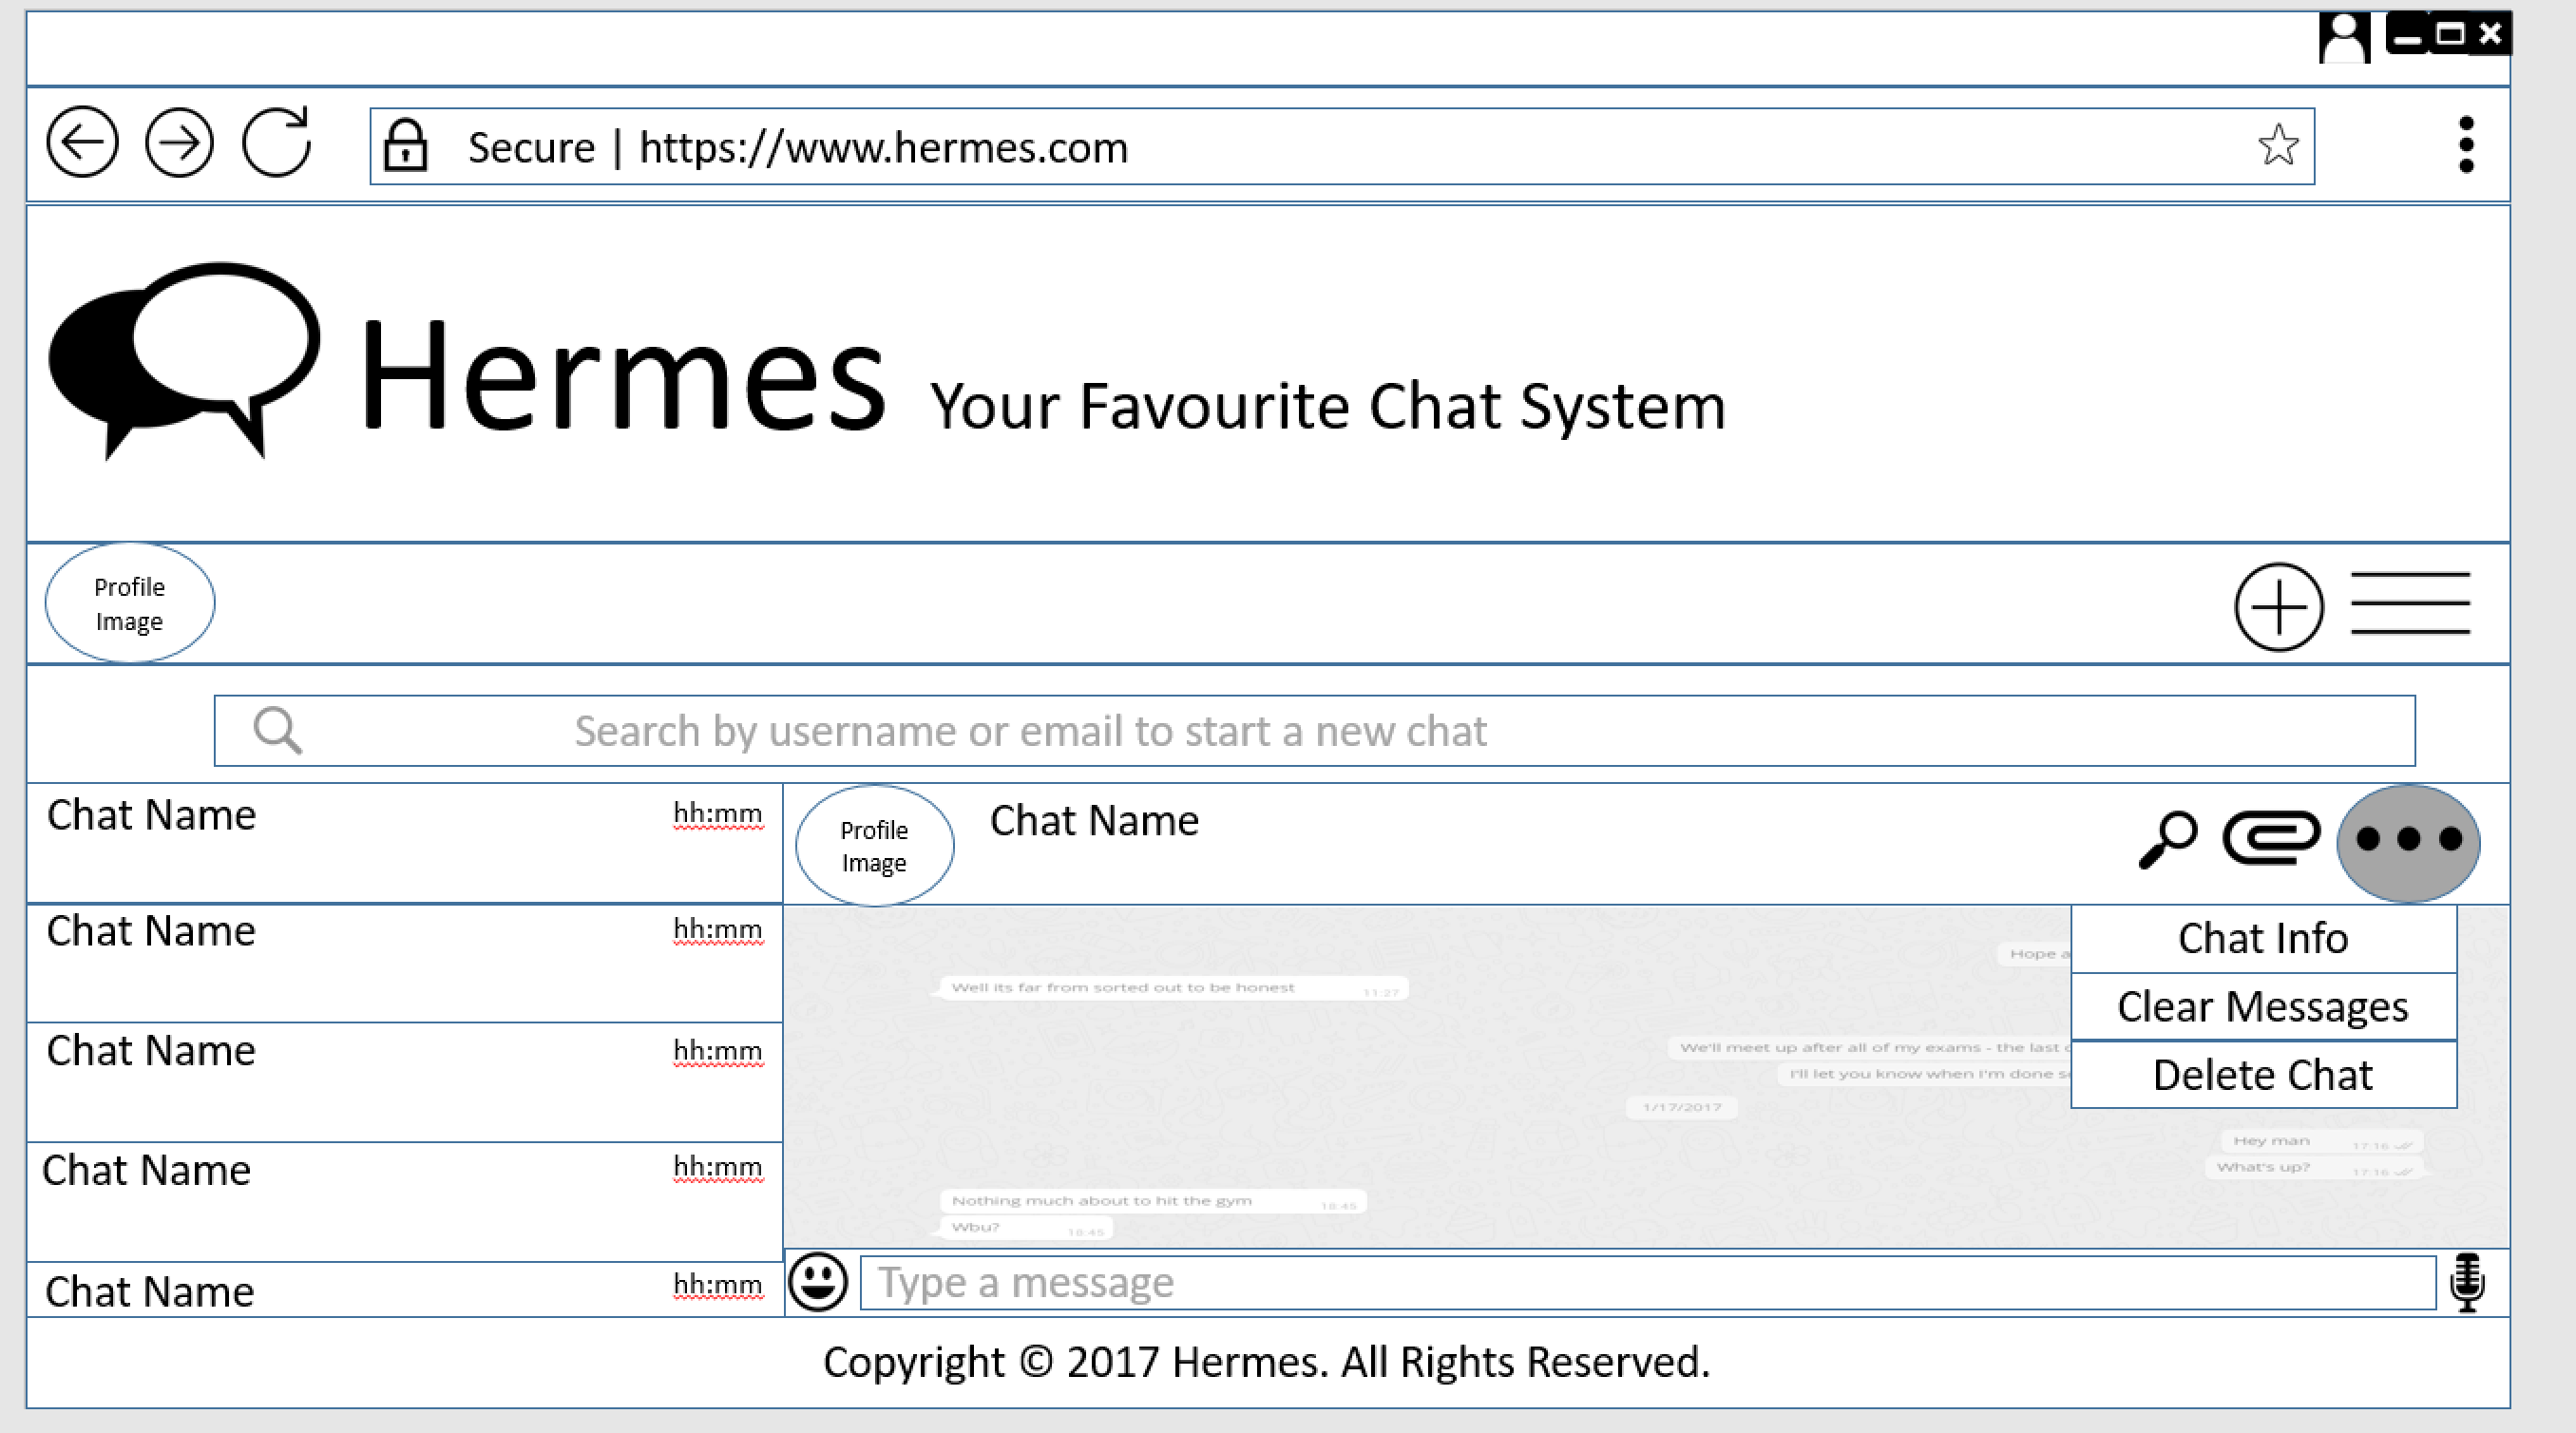
\includegraphics[width=10cm, height=5cm]{w6}
\end{center}

\subsection{Android Application Prototype}
\begin{center}
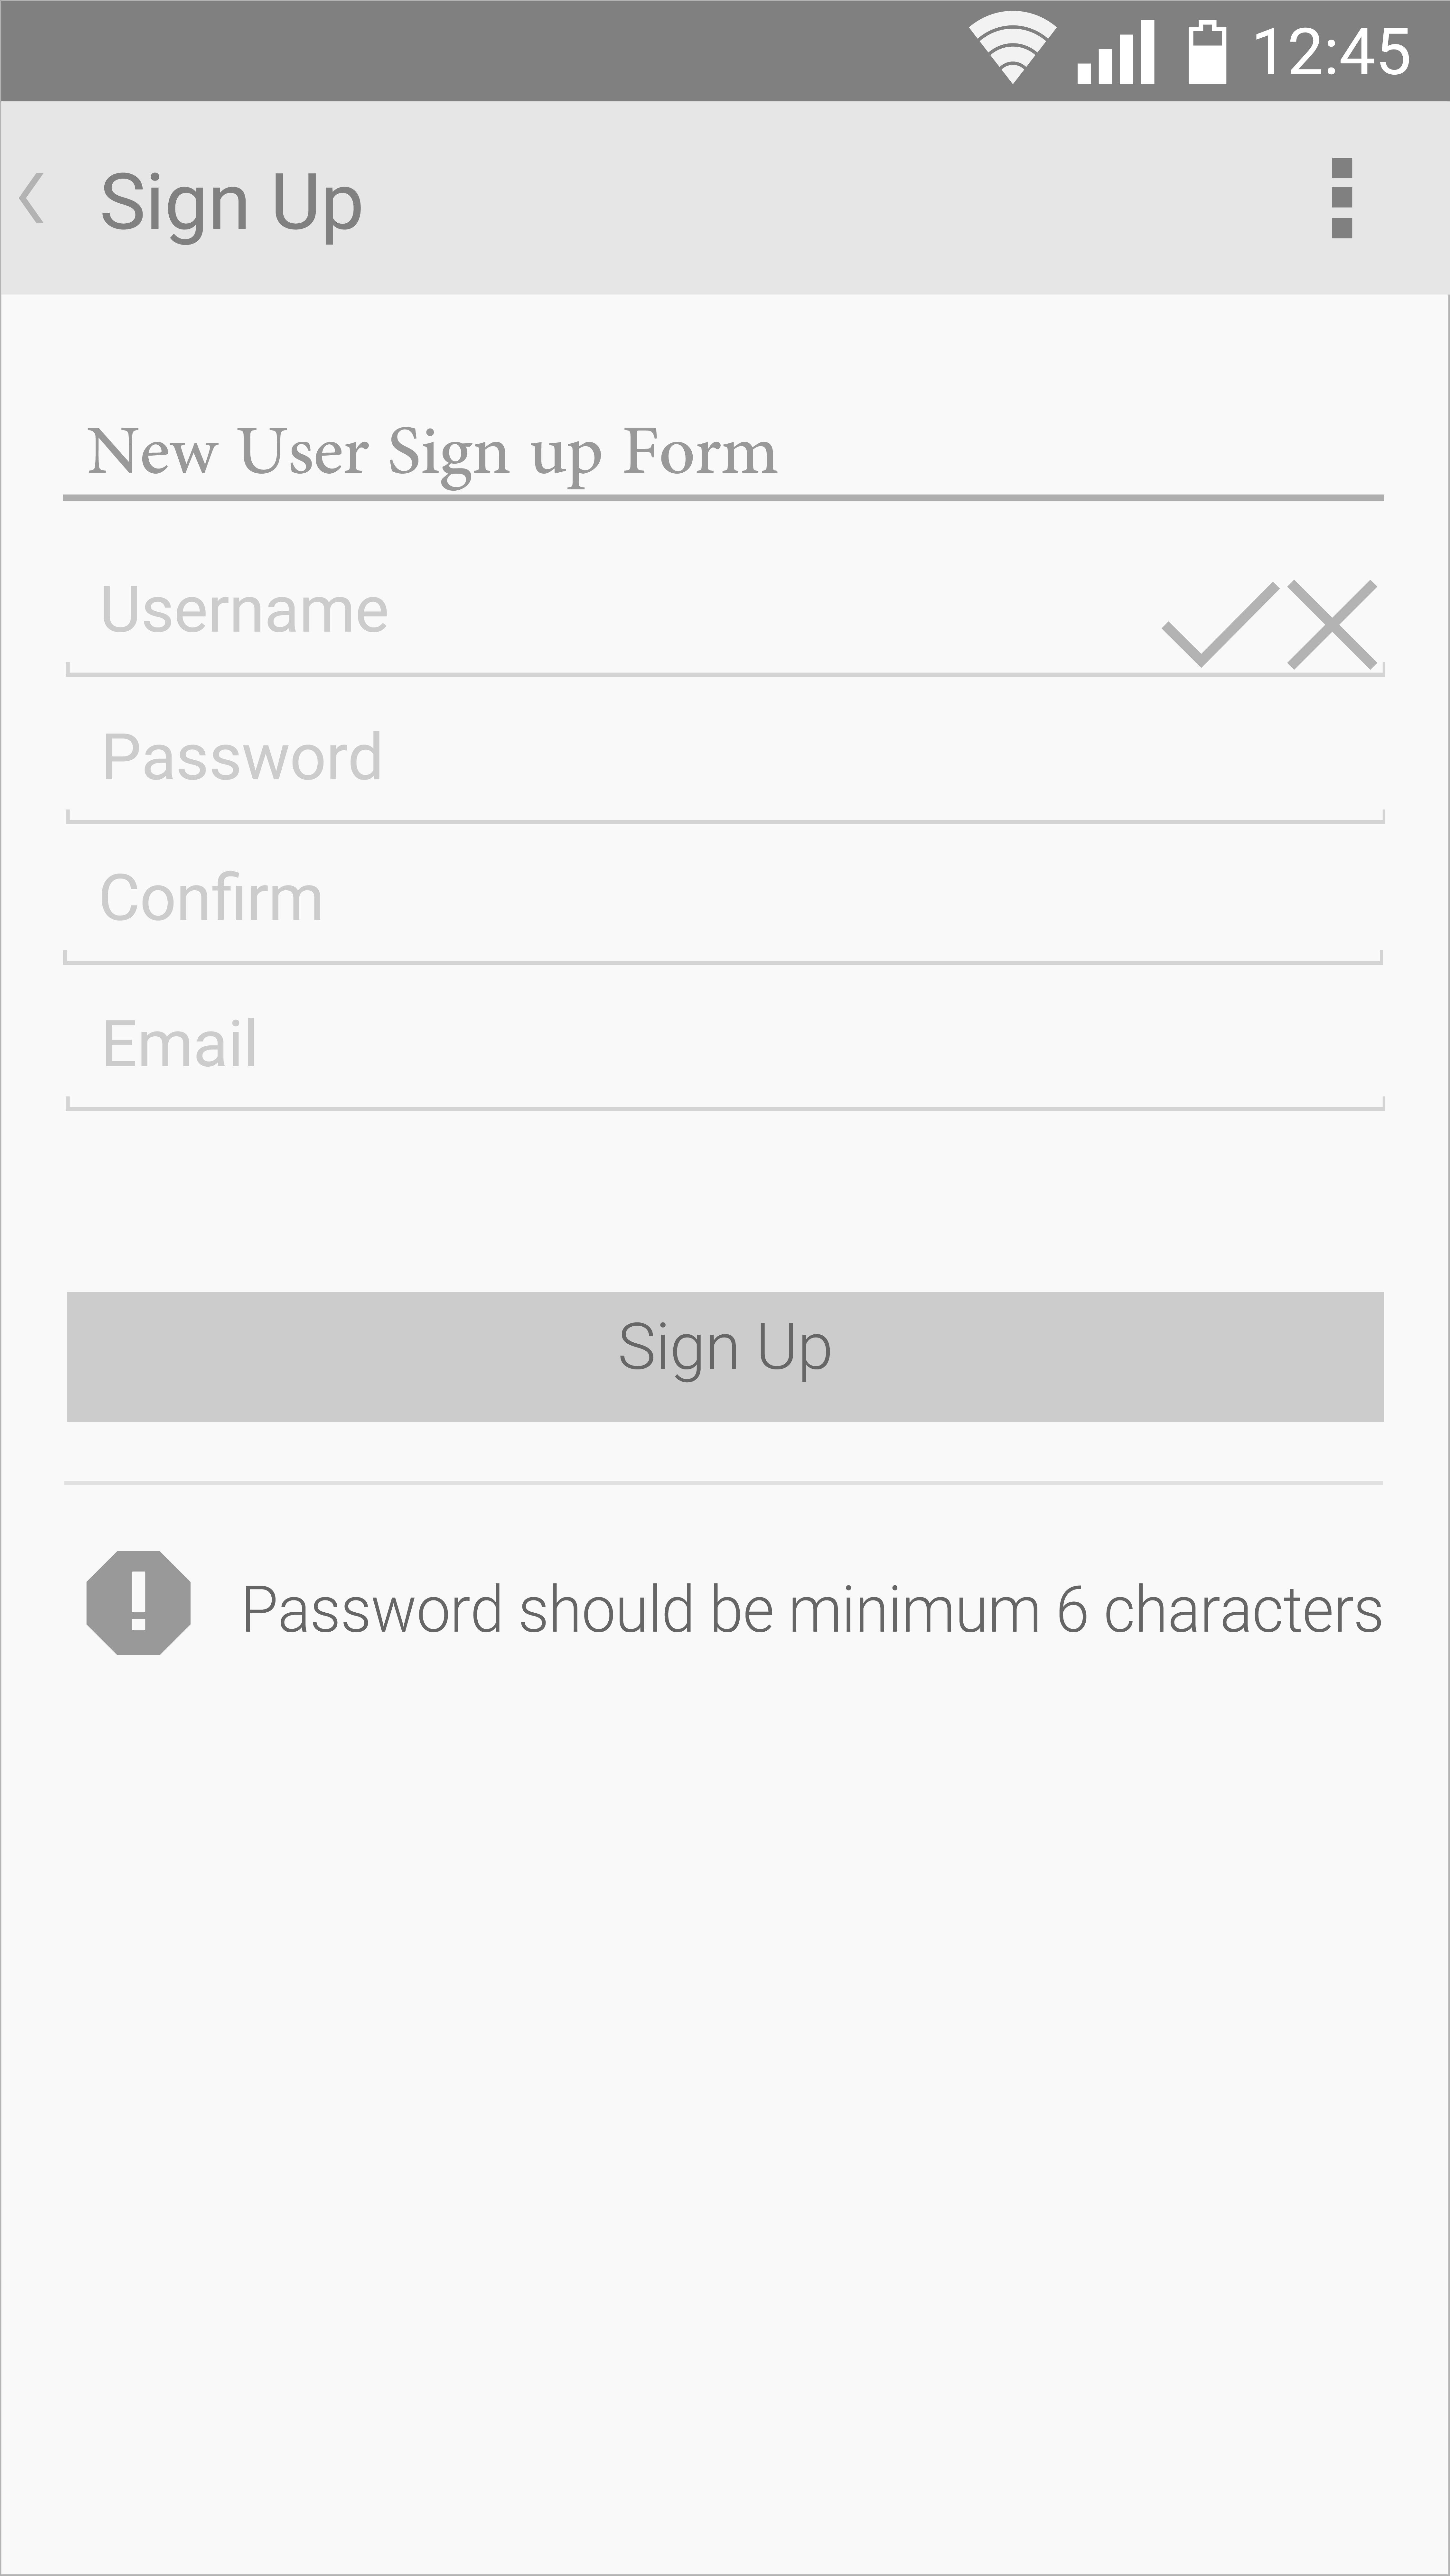
\includegraphics[width=5cm, height=10cm]{SignUp}
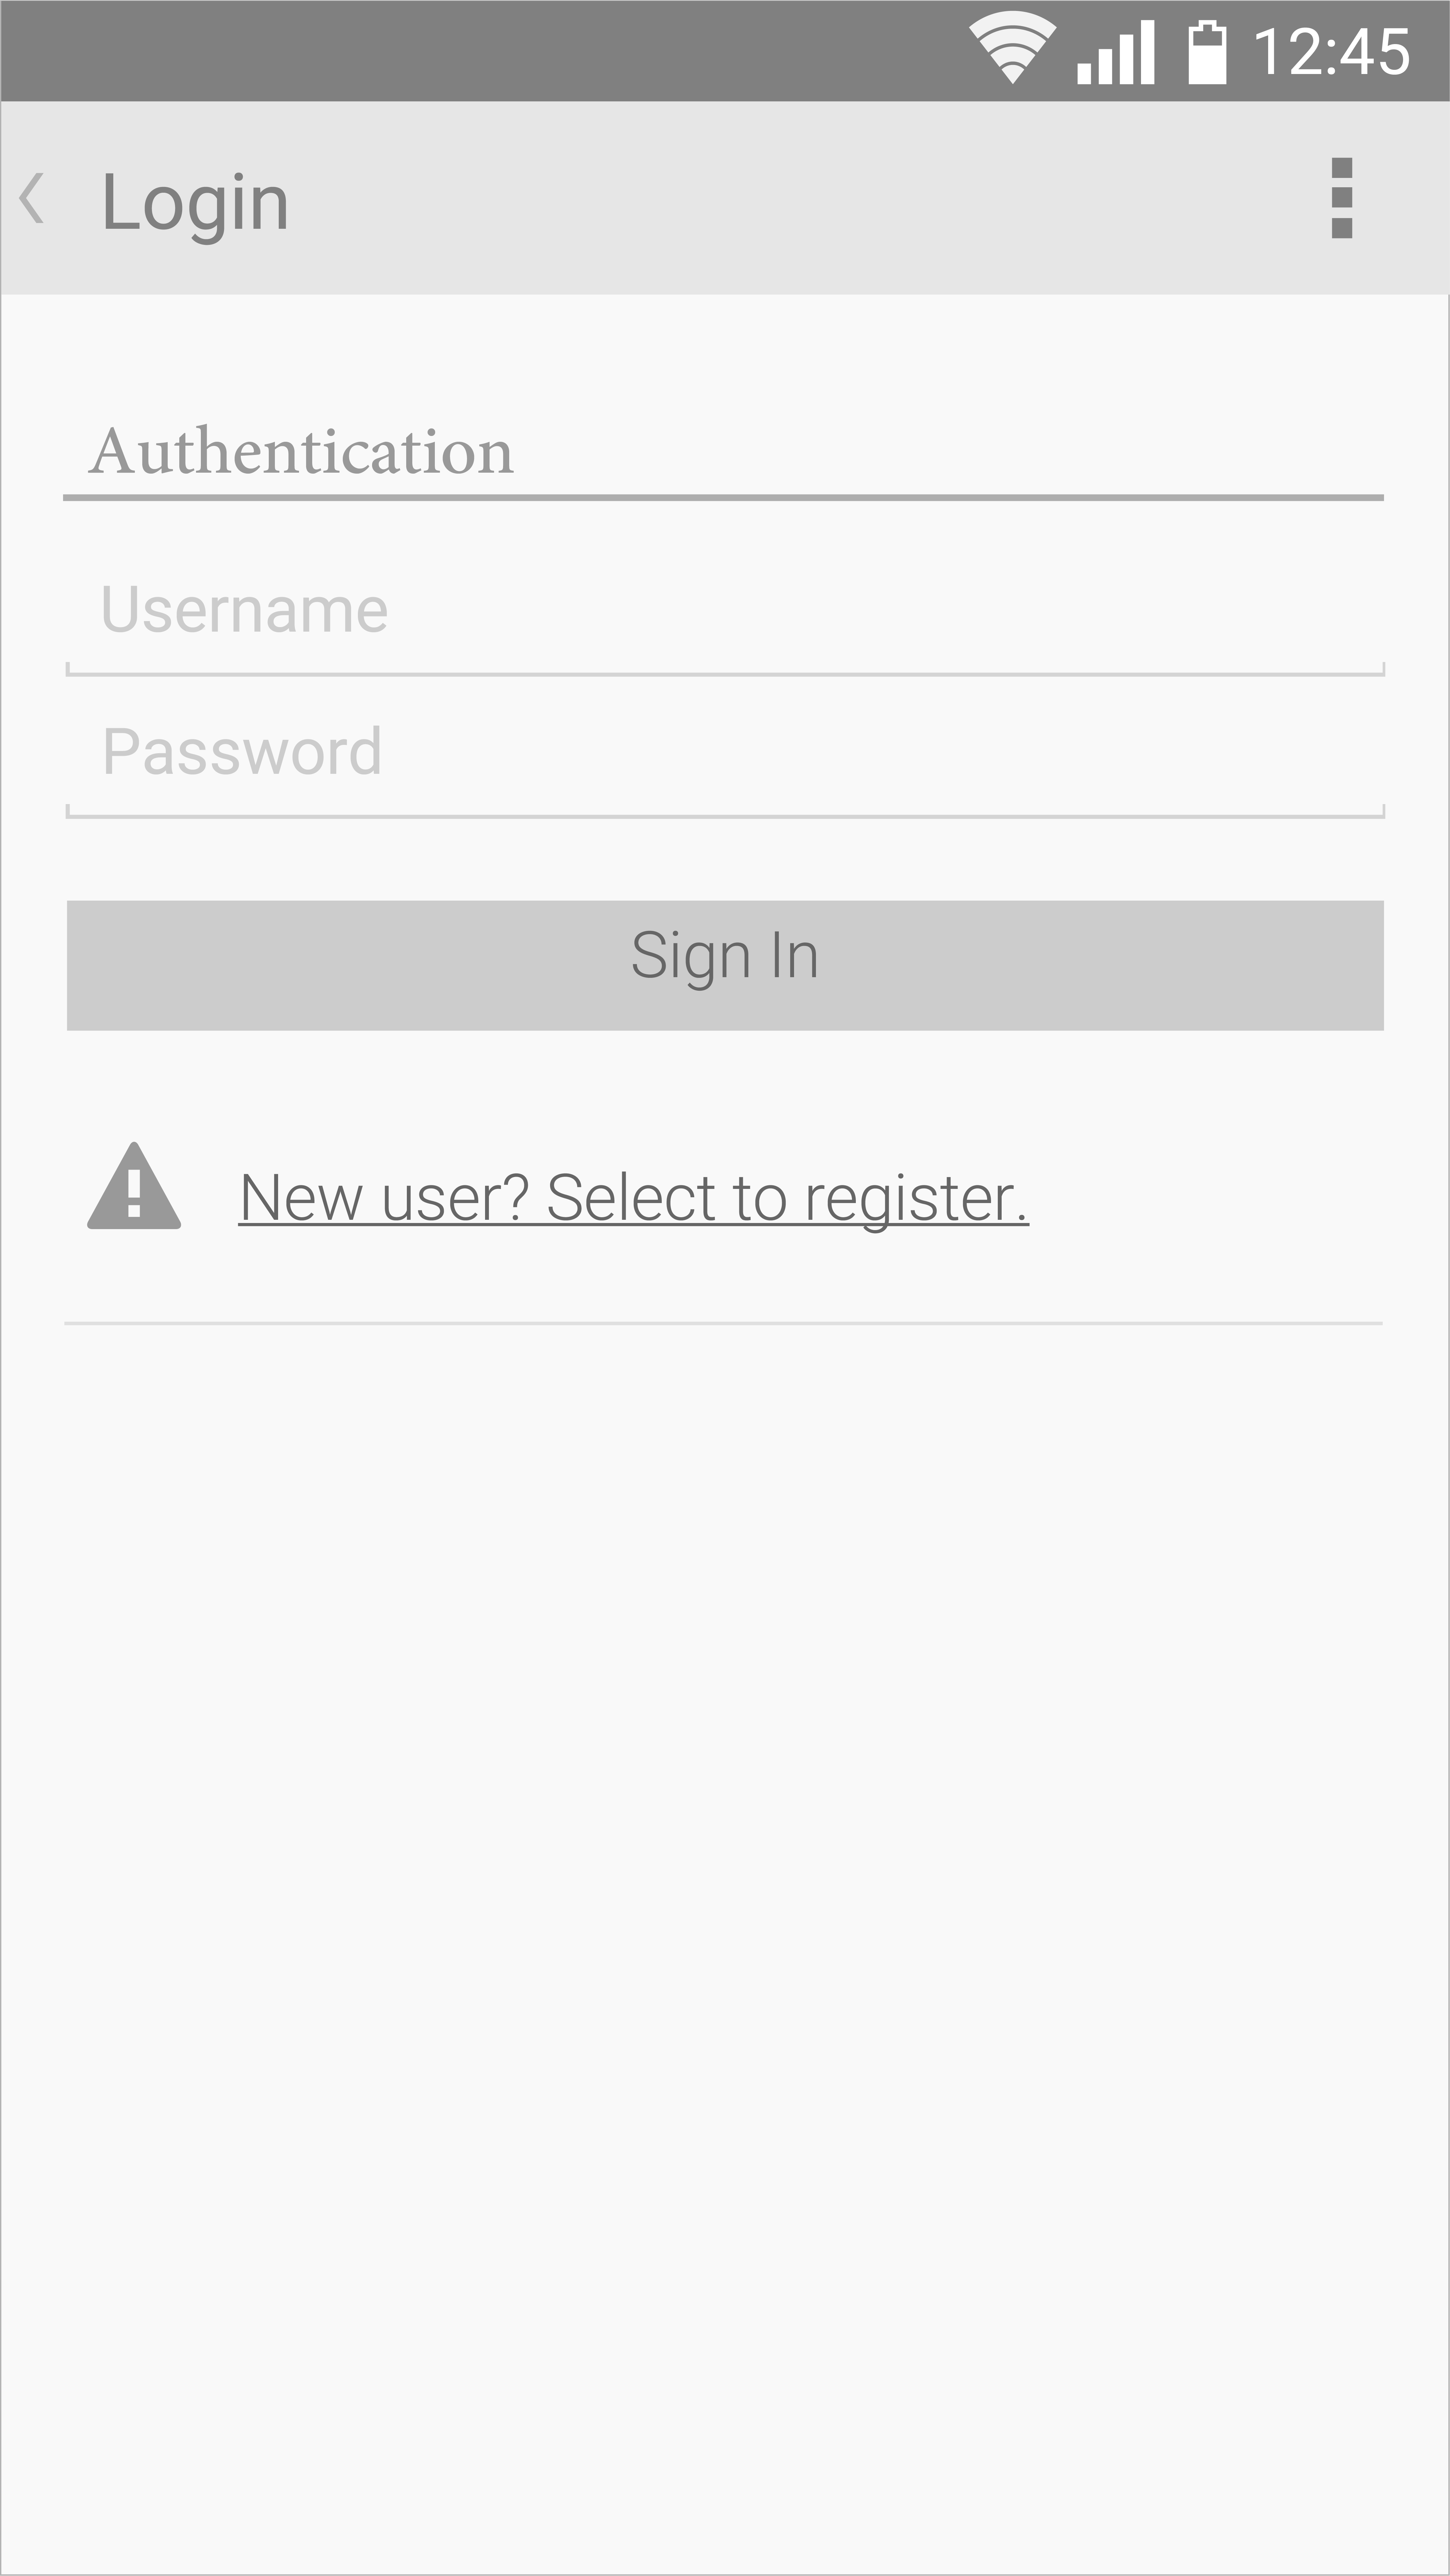
\includegraphics[width=5cm, height=10cm]{SignIn}
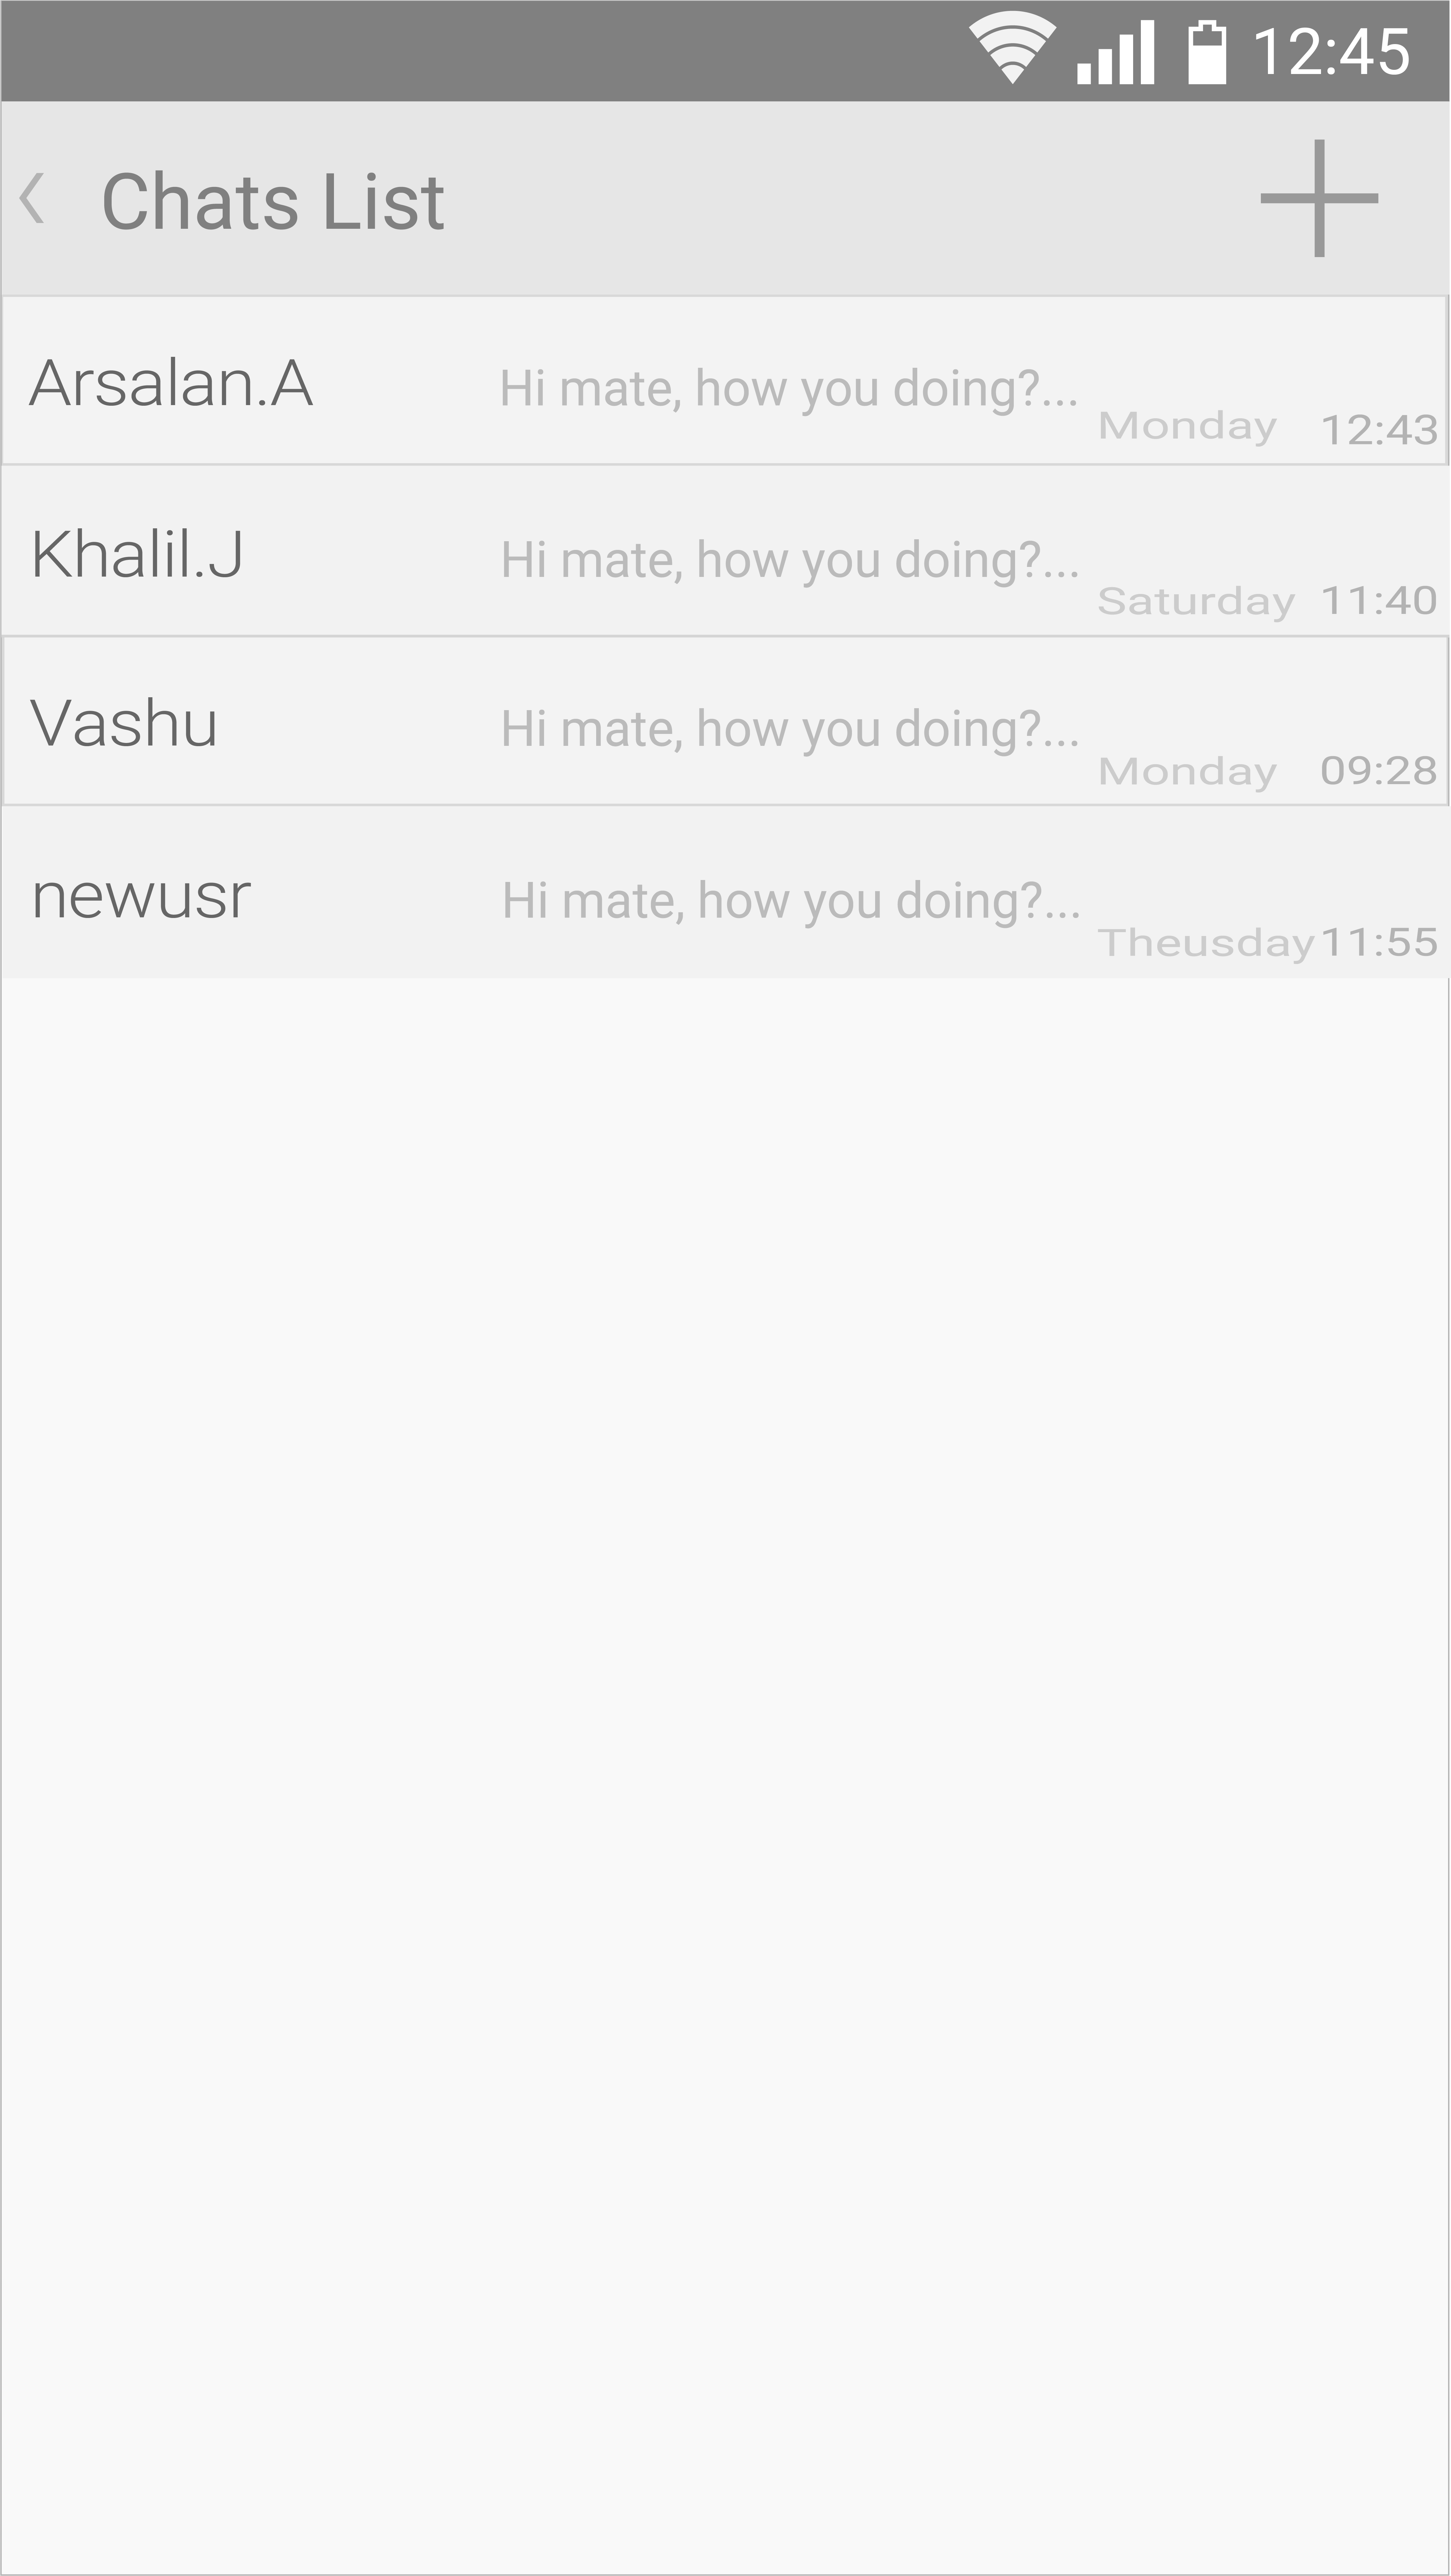
\includegraphics[width=5cm, height=10cm]{ChatList}
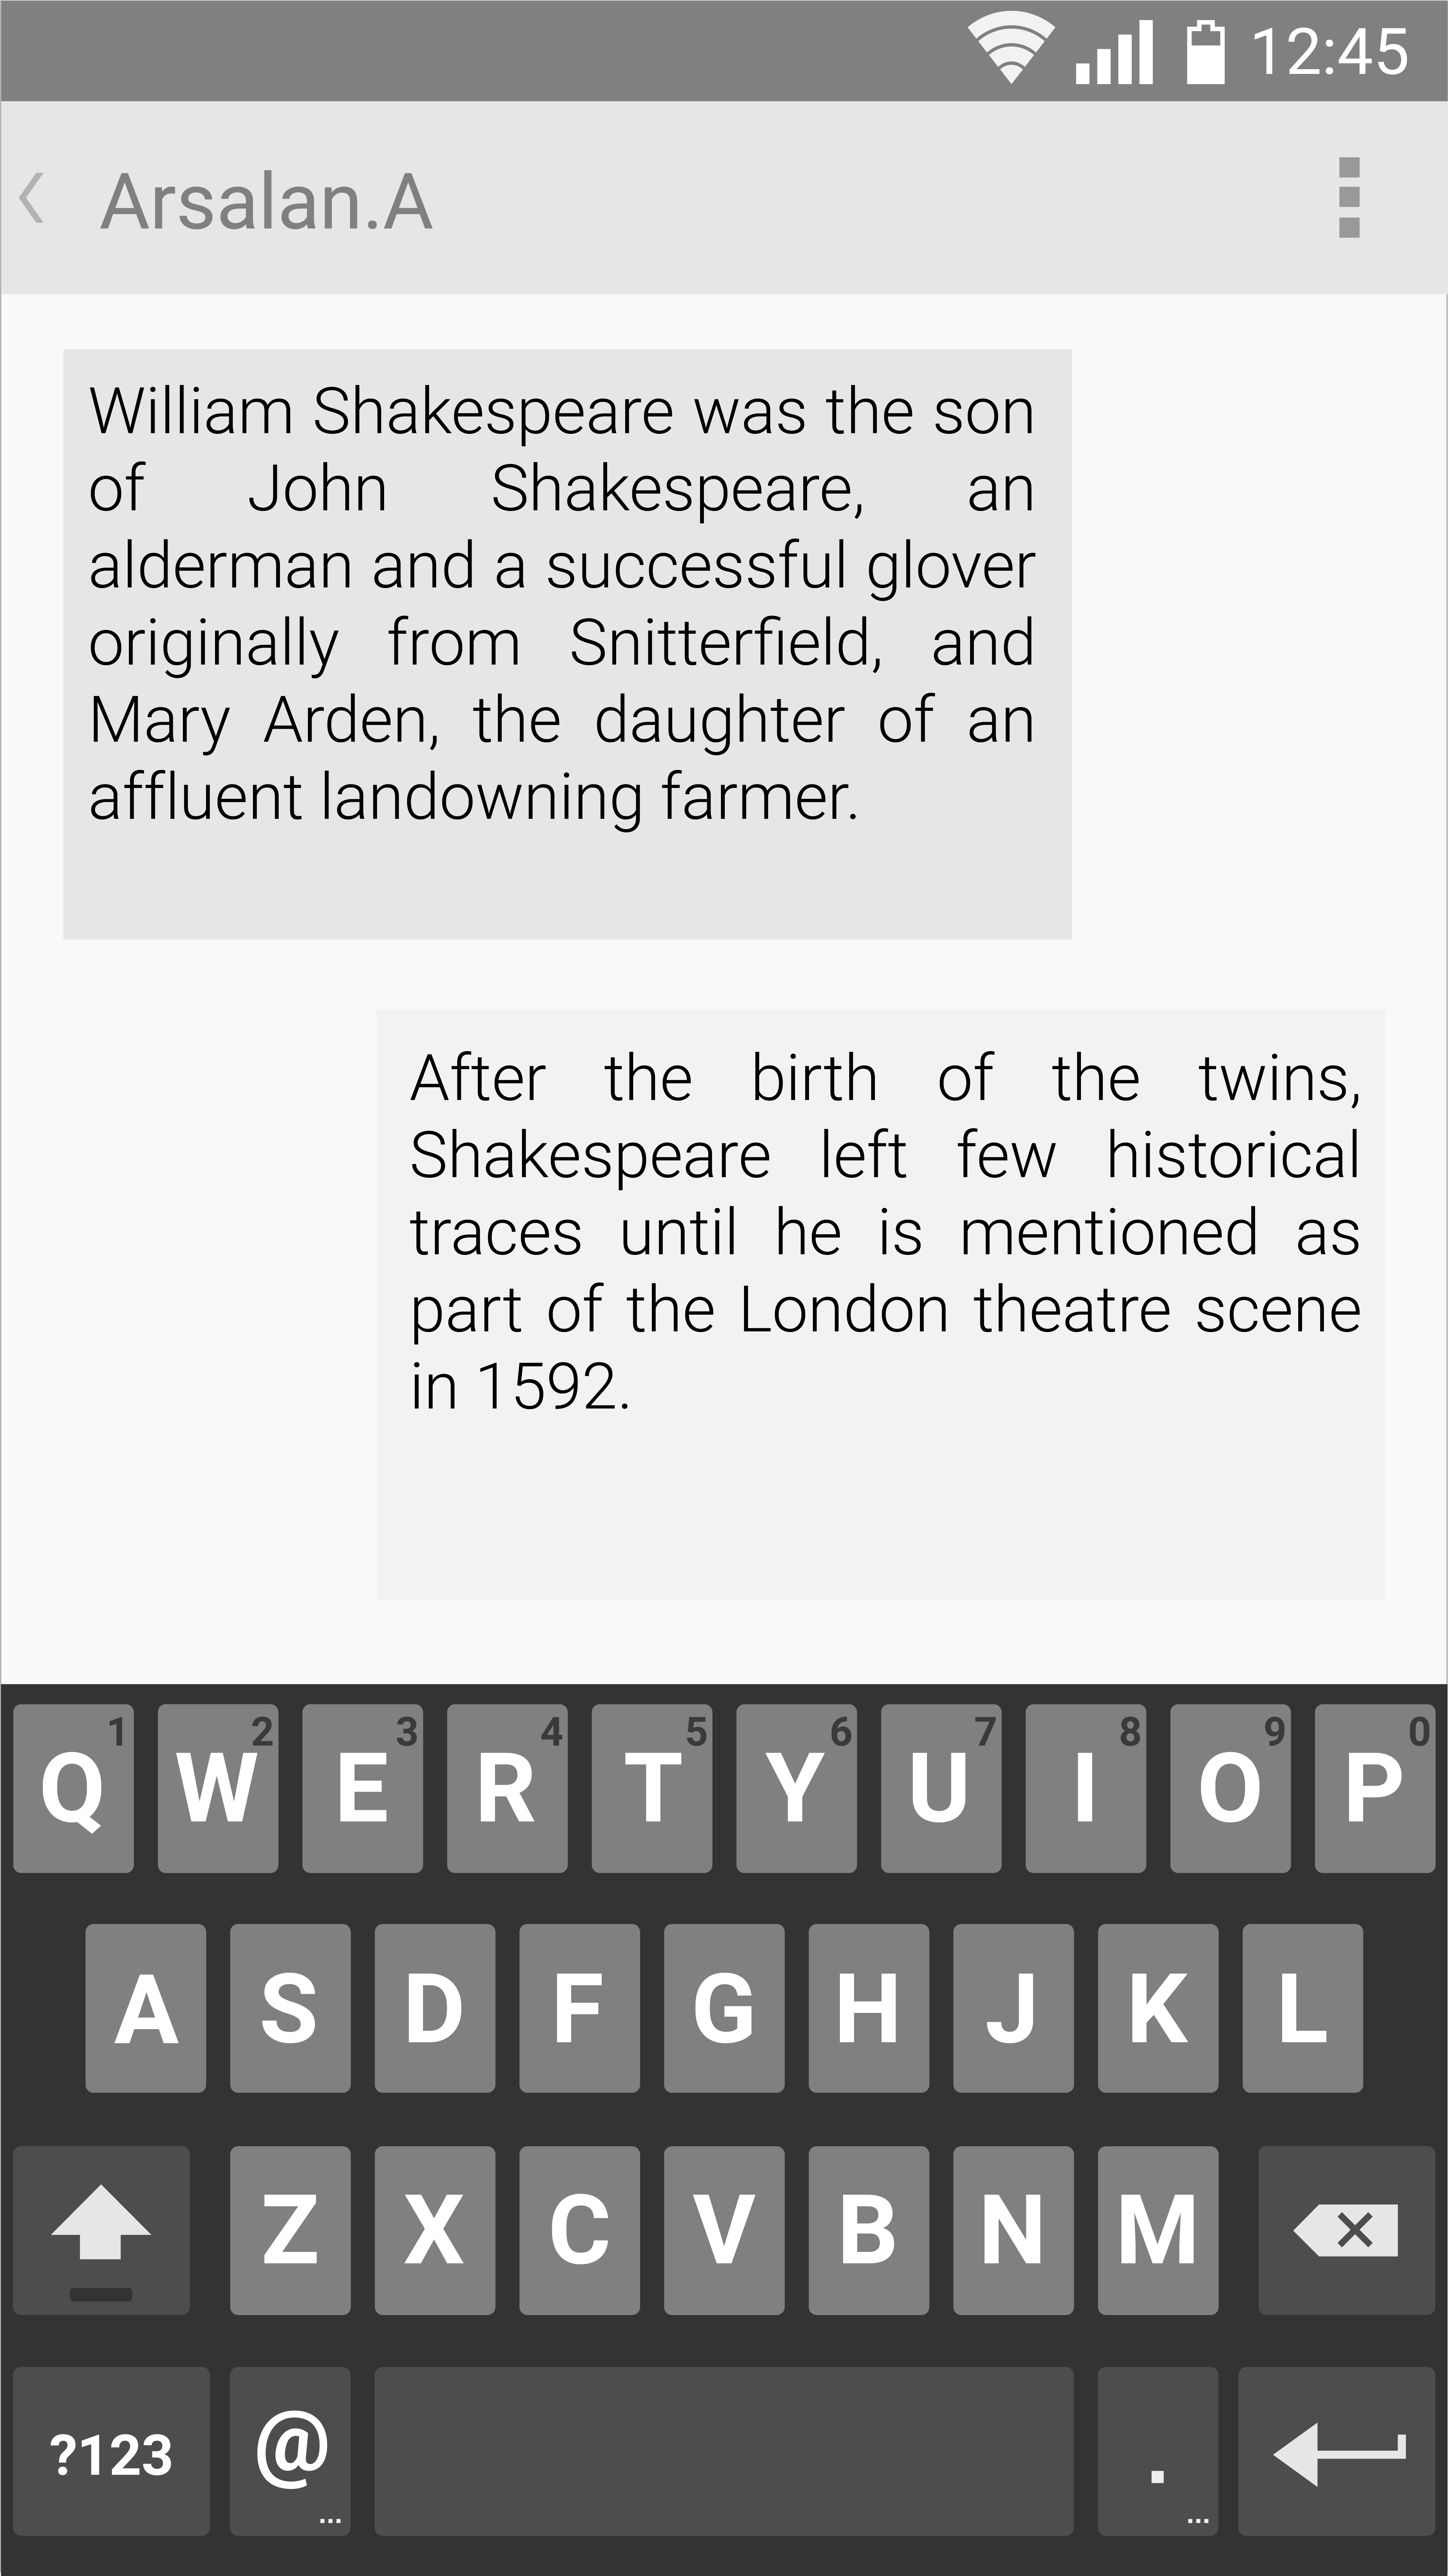
\includegraphics[width=5cm, height=10cm]{Messages}
\end{center}

\newpage
\section{Methodology and Framework}
\subsection{Four Key Principles of Agile}
‘Agile project management is an evolution to the agile software development movement.’ There are four key principles for the Agile manifesto as below \cite{Agile-Scrum}: \par
\begin{itemize}
\item \textbf{Individuals and interactions over processes and tools}: this is extremely important to this project as individuals who are the developers of the system to interact efficiently with each other instead of having commitments to specific processes and tools. 
\item \textbf{Working software over comprehensive documentation}: ensuring right construction of the software system which will be fully functional instead making a comprehensive documentation. This will ensure a delivery of a working system in the end. 
\item \textbf{Customer collaboration over contract negotiation}: developers have close connection with the user to better comprehend user’s requirements from the early to final stages of the software life cycle. 
\item \textbf{Responding to change over following a plan}: the software system should be adaptable to account for changes in resources and technologies over time. Therefore, following a plan is not ideal in Agile as new requirements may arise and thus the plan will change. 
\end{itemize}

\subsection{Scrum:Sprints Plan}
\begin{enumerate}
\item \textbf{Designing interfaces for both platforms based on the wire-frames}:
the Wire-frames were designed to provide a standard for both platforms to keep the consistency of the system and improves the user experiences. However, we have some differences between platforms regarding their natures. Additionally, it helped the further designing and future implementation because of visual presentation of the system which made imagination and user needs more visible. 
\item \textbf{Design and implement the database and connect the two platforms to the actual database}: 
for this Iteration, the goal was to make the database up and running on the server by starting to establishing the connection between both platforms and the server. This will enable testing the system through adding, selecting, updating and deleting data from the database. ACID properties of the database and system could be measurable and meaningful after completing this section and would provide a reasonable prototype for the customer to find out what could be the other needs and requirements of the system.
\item \textbf{Creating stored procedures and configuring both platforms to use the same SPs}:
stored procedures are extremely important, especially for systems which are implemented over different platforms. Their use brings a variety of advantages for the system, some of the most important ones are as follows, providing consistency for interactions with the database because both platforms use the same SPs which will dictate platforms to follow the rules and business work flow of the system in a more secure manner. Secondly, because it sets once a time in the database and instantly will reflect into platforms, it will increase scalability and re-usability of the system in a great amount. Lastly, but not the least important one, it will improve the security of the system by suppressing and preventing SQL commands or possibly SQL Injection attacks by hiding and adding another layer for accessing data and running commands over the database.
\item \textbf{Finalise interactions to server and start considering some test cases to find possible errors}:
for satisfying the consistency and integrity of system interactions to the server side playing a crucial role. Also, some testing on server side could be more efficient because will detect possible errors which would be revealed through testing in both platforms separately. Finally, need to run some sets of possible inputs and check the result given by system to find some unknown error either in back-end or front-end possibly. Errors should be found and fixed before releasing the software. Undiscovered errors after publishing the software will indicate a failure so the errors are found earlier e.g. during the implementation phase, the better. 
\item \textbf{Examine system performance/efficiency and consistency over real workload of the system}:
performance and efficiency examination took place as the last iteration to verify and observe the system in terms of workload and transaction stress. The system will be tracked over the system's load to see if there is any flaw exist in the real-time use of the chat system. Flaws could have different types include running time or inconsistency in working with the chat system on peak time which might be caused by incorrect way of designing the database or SQL commands that were used. For example, these deficiencies could be resulted by not optimising queries for returning data or validation at the server side or even find some weaknesses in either of platforms in case of several users using the application at the same time.    
\end{enumerate}

\newpage
\section{Software Testing}
\begin{center}
 \begin{longtable}{| p{1.5cm} | p{1cm} | p{1.5cm} | p{2.5cm} | p{1cm} | p{1cm} | p{2.5cm} |} 
 \hline
 FR or Case & Test ID & Type & Description & Date & Result & Comments\\ [0.5ex] 
 \hline\hline
Register User & T1 & Functional & Fill in the registration form and create a new user. & 27-03-2017 & Pass & \\
\hline
Validation of Username and Password & T2 & Functional & Validate the username and password entered by the user. & 27-03-2017 & Passed &\\
\hline
Login User & T3 & Functional & Feed the username and password, validate them and authenticate the user. & 27-03-2017 & Passed &\\
\hline
Send Message & T4 & Functional & Insert a user written message to the server database. & 27-03-2017 & Failed & There was an error with PHP file concerned with adding messages to the database. \\
\hline
Send Message & T5 & Functional & Insert a user written message to the server database. & 27-03-2017 & Passed & Test passed after correction of the PHP file. \\
\hline
Search User & T6 & Functional & Search for user by username to initiate a new chat. & 27-03-2017 & Failed & Failed due to wrong usage of OnKeyPress event. \\
\hline
Search User & T7 & Functional & Search for user by username to initiate a new chat. & 27-03-2017 & Passed & Used the OnKeyUp event instead. \\
\hline
Initiate New Chat & T8 & Functional & If the user selects a new user and sends the first message, then create a new chat in the database. & 27-03-2017 & Passed &\\
\hline
Chat List Loading & T9 & Functional & Load a list of all chats associated with the current user. & 27-03-2017 & Failed & Logical error due to use of a wrong PHP function. \\
\hline
Chat List Loading & T10 & Functional & Load a list of all chats associated with the current user. & 27-03-2017 & Passed & Correct function was used instead. \\
\hline
Receive Messages & T11 & Functional & Load Messages for the current user that are inserted in the database in real-time. & 27-03-2017 & Passed & Works only if the application or website is open. Push notifications are not implemented. \\
\hline
\end{longtable}
\end{center}

\newpage
\section{Peer Assessment Marking Criteria}
\subsection{Marks Distribution}
\subsubsection{Group Meetings (20\%{})}
 \begin{tabular} {| c | c |}
  \hline
  Attendance. & 4\%{} \\
  \hline
  Involvement in discussions during meetings. & 4\%{} \\
  \hline
  Suggesting new ideas or techniques to enhance development. & 4\%{} \\
  \hline
  Listening to others’ ideas and suggestions. & 4\%{} \\
  \hline
  Be efficient. & 4\%{} \\
  \hline
 \end{tabular}

\subsubsection{Communication and Collaboration (35\%{})}
 \begin{tabular} {| c | c |}
  \hline
  Oral and verbal communications. & 5\%{} \\
  \hline
  Inform group members in case of emergencies. & 5\%{} \\
  \hline
  Update team members of individual progress. & 5\%{} \\
  \hline
  Helping team members when necessary. & 5\%{} \\
  \hline
  Respect to the project (caring). & 5\%{} \\
  \hline
  Respect to the team members. & 5\%{} \\
  \hline
  Flexibility. & 5\%{}\\
  \hline
 \end{tabular}

\subsubsection{Individual Tasks and Deliver-ables (45\%{})}
 \begin{tabular} {| c | c |}
  \hline
  \multicolumn{2}{|c|}{Complete your assigned tasks or deliver-ables:} \\
  \hline
  According to specifications. & 15\%{} \\
  \hline
  With the required quality. & 15\%{} \\
  \hline
  Within the time frame . & 15\%{} \\
  \hline
\end{tabular}

\subsection{Formula}
The following formula was used to calculate each individual’s final mark as follows: \newline
Final mark = (individual mark / the sum of all members’ individual marks) * 100. This will give a mark out of 100 split between team members based on the marking schema. 
If all members contributed equally, they will get 25\%{} each in the case of four members. 
Also, a member could get higher than 25\%{} e.g. if they secure a better percentage than others as specified in the previous section. 


\end{appendices}

\end{document}
